Modeling the transition between different nuclear fuel cycles provides 
information on the quantity and timing of various materials to meet 
specific objectives, such as providing fuel for reactors to meet a 
prescribed energy demand. 
This work models potential transitions from the 
current fleet of \glspl{LWR} in the US to advanced reactors to quantify the 
resources required to support the transition. 
This work considers a variety of transition scenarios, primarily grouped 
into once-through and recycle scenarios. Sections \ref{sec:once-through-methods}
and \ref{sec:recycle-methods} describe more specific details of the 
scenarios. However, there are multiple details that apply to all of 
the scenarios, which are described here. 

We used \Cyclus \cite{huff_fundamental_2016} to model the transitions, 
with archetypes from the \Cycamore library \cite{carlsen_cycamore_2014}
defining the non-reactor facilities. Each scenario models the fuel 
cycle between 1965-2090 using a time step of one month. 
The transition from \glspl{LWR} 
to advanced reactors begins in January 2025, so the energy generated by 
\glspl{LWR} in 2025 is the basis for the energy demand in each scenario.  
Many of the 
current plans for \gls{HALEU}-fueled reactors do not have these reactors 
deployed until the late 2020s \cite{nichol_current_2021} through \gls{ARDP} 
and other programs. selecting 2025 as the transition 
start time for this work provides a bounding case for 
an aggressive deployment of these reactors. 

Information about the US \glspl{LWR} is from the \gls{IAEA} \gls{PRIS} 
database \cite{noauthor_power_1989}, providing the start dates and 
power outputs (MWe) for all of the \glspl{LWR} and end 
dates for select \glspl{LWR}. The \gls{PRIS} database only contains end dates 
for reactors that are shut down before the publication of the 
database each year. Reactors still operating in December 2020  
(the year of the database used for this work) lack an end date 
in the \gls{PRIS} database and are assumed to operate until 
their current operating license expiration date, obtained from 
\cite{nuclear_energy_institute_us_2021}. This work considers only 
reactors in the \gls{PRIS} database with a power level above 400 MWe 
to avoid including prototype and research reactors present in the database. 
Approximate masses for fuel used in the cores of the \glspl{LWR} were obtained 
from literature \cite{todreas_nuclear_2012,cacuci_handbook_2010}. 

This work considers multiple metrics of the fuel cycle transitions: 
the energy produced, the number of reactors deployed, the 
uranium requirements (both enriched uranium required for fuel and feed uranium 
to produce enriched uranium), 
the \gls{SWU} capacity required to produce the enriched uranium, and the 
amount of waste produced. Comparing each of these metrics provides 
information on the material requirements of the transition, which further 
informs the capacity and number of facilities required to support 
the transition. The natural 
uranium usage and waste production are two of the metrics used in the 
\acrfull{ES} 
\cite{wigeland_nuclear_2014}, and the mass of enriched uranium was the 
primary result of the work by Dixon et al. \cite{dixon_estimated_2022}. 
The previous use of these fuel cycle metrics contributed to the development 
of this list of material requirements to compare.

\section{Advanced reactor modeling} \label{sec:reactor_methods}
This work considers three advanced reactors: the \gls{USNC} \gls{MMR}, 
\cite{mitchell_usnc_2020,noauthor_usnc_2021}, the X-energy Xe-100 
\cite{mulder_overview_2021}, and the NuScale VOYGR reactor
\cite{nuscale_chapter_2020-1,reyes_nuscale_2021,reyes_correction_2022}. 
Table \ref{tab:reactor_summary} provides some design parameters 
of each of these reactors. The values in this table closely match the 
design information about each reactor that is available through open-source 
information. The 
\gls{USNC} \gls{MMR} and X-energy Xe-100 reactors require \gls{HALEU}, 
but the NuScale VOYGR requires \gls{LEU} with a similar enrichment level 
to current \gls{LWR} fuel. This work 
includes the NuScale VOYGR, despite not requiring \gls{HALEU} fuel, 
because the \gls{NRC} granted it design approval \cite{world_nuclear_news_nuscale_2021} 
and it is of the author's personal opinion that it is very likely to be deployed 
along-side \gls{HALEU}-fueled 
reactors. Including the VOYGR reactor in the transition scenarios provides 
insight into how the deployment of \gls{HALEU}-fueled and non-\gls{HALEU}-fueled 
advanced reactors in tandem affects the material requirements of the transition. 

\begin{table}[ht]
    \centering
    \caption{Advanced reactor design specifications.}
    \label{tab:reactor_summary}
    \renewcommand{\arraystretch}{1.5}
    \begin{tabular}{p{3.5cm}p{3cm}p{3cm}p{3cm}}
        \hline
        Design Criteria & \gls{USNC} \gls{MMR} \cite{noauthor_usnc_2021} & 
        X-energy Xe-100 \cite{mulder_overview_2021} & NuScale VOYGR 
        \cite{nuscale_chapter_2020-1,reyes_nuscale_2021,reyes_correction_2022}\\
        \hline
        Reactor type & Modular HTGR & Modular HTGR & SMR\\
        Power Output (MWth) & 15 & 200  & 250 \\
        Capacity Factor & 100\% & 95\% & 95\% \\
        Enrichment (\% $^{235}U$) & 19.75 & 15.5 & <4.95 \\
        Cycle Length (yrs) & 20 & online refuel & 1.5\\
        Number of cycles & 1 & 6 & 3\\
        Fuel form & UO$_2$ \gls{FCM} compacts & UCO \gls{TRISO} pebbles & UO$_2$ pellets\\
        Discharge fuel burnup (GWd/MTU) & 82 & 168  & 45 \\
        Reactor Lifetime (yrs)& 20 & 60 & 60 \\
        \hline
    \end{tabular}
\end{table}

The refueling scheme for each reactor includes 
the cycle time, the refueling time, and the mass of fuel put into the reactor 
at each refueling. The fuel mass required by 
each reactor type was calculated based on the reactor thermal power, 
cycle length, and burnup:

\begin{equation}
    \text{mass [kg] = }\frac{\text{Power [MWth]}* \text{cycle 
    length [d]} * \text{number of cycles}}{\text{burnup [MWd/kg]}}
    \label{eq:fuel_mass}
\end{equation}

\noindent Eq. \ref{eq:fuel_mass} calculates the mass of uranium required 
in the core. To calculate the total mass of the fuel (including the non-heavy 
metal in the fuel) this value was divided by the mass fraction of 
uranium in the fuel form for the reactor. Any non-uranium bonded components 
of the fuel, such as silicon-carbide in \gls{TRISO} particles, were 
not considered in the mass. This methodology assumes that the 
uranium and uranium-containing fuel components would be the limiting 
factor in the fuel cycle and other fuel components would be available as 
needed. 

The \gls{MMR} does not undergo refueling; the initial core
burns for the entire lifetime of the reactor \cite{mitchell_usnc_2020}. 
Therefore, the \gls{MMR} has a cycle length that 
matches the reactor lifetime. Additionally, the refueling mass for the
\gls{MMR} is zero. The Xe-100 undergoes online refueling operations, with 
each \gls{TRISO} pebble passing through the reactor six times before 
discharge \cite{mulder_overview_2021}. Every seven months about 1/6th 
of the pebbles in the core are expected to be discharged. The Xe-100 
refueling is modeled as a refueling time of zero months and a 
replacement of 1/6th of the core mass every seven months. 
The VOYGR contains 37 fuel assemblies, with three different enrichment 
levels \cite{nuscale_chapter_2020-1}. Each refueling replaces 13 fuel 
assemblies, with the middle assembly replaced at every refueling. 
Therefore 13/37th of the core mass is replaced at each refueling. 
The fuel enrichment used is an average of the assembly enrichments 
presented in \cite{nuscale_chapter_2020-1}. NuScale reports that a refueling 
outage for the VOYGR will take ten days \cite{nuscale_nuscale_2022}. 

Fresh fuel recipes for the advanced reactors are based on the 
defined fuel form for each reactor using the appropriate uranium isotope 
ratio for enrichment. Both the \gls{MMR} and VOYGR are intended to be built 
in sets (2 \gls{MMR} per site \cite{noauthor_usnc_2021} and up to 12 VOYGR 
units per site \cite{reyes_nuscale_2021}), but in this study every reactor 
design is treated 
on a single unit basis. Therefore, the number of reactors built in each 
of the transitions does not represent the number of unique sites required 
to build the reactors. All cores modeled are assumed to be equilibrium cores; 
this work does not consider start-up cores or the transition to equilibrium. 

To properly account for the capacity factor of each reactor, the power output 
(in MWe) of each reactor was multiplied by the capacity factor and explicit 
modeling of outages was removed. This methodology was applied to the 
advanced reactors and the current fleet of \glspl{LWR}, which were assumed 
to operate with a 92.66\% capacity factor based on the last five years of 
fleet-averaged capacity factors 
\cite{us_energy_information_administration_electric_2022}. 
By removing explicit modeling of outages, the outages do not artificially affect 
the capacity factors. The operating cycle of the \glspl{LWR} and VOYGRs 
was extended by 1 time step, to ensure that these facilities received fuel 
on the same schedule as if the outages were explicitly modeled. 

\section{Once-through fuel cycle} \label{sec:once-through-methods}
Figure \ref{fig:once-through_fuel_cycle} shows the flow of material through 
the modeled once-through fuel cycles. The once-through fuel cycle models 
material from the mine to final disposal in a repository. The 
``Advanced Reactor'' node in Figure 
\ref{fig:once-through_fuel_cycle} represents any subset of the advanced 
reactors (Xe-100s, \glspl{MMR}, and VOYGRs) included 
in the scenario. This model assumes that all enriched uranium is produced 
by enriching natural uranium; this work does not consider downblending \gls{HEU} 
to produce \gls{LEU}. 
This fuel cycle is a simplified version of the modeled fuel cycle in 
\cite{bachmann_enrichment_2021}, removing steps in the fuel cycle that 
do not affect the reported results. Removing some of the steps simplified 
the models from a user standpoint and reduced the size of the \Cyclus 
output file, facilitating data analysis. The transition from the 
\glspl{LWR} to the advanced reactors begins in 2025. Each of the non-reactor 
facilities have an unlimited capacity to produce or process materials,
to prevent material unavailability from influencing the results. 
This methodology has previously been applied to transition analysis 
\cite{djokic_application_2015}. Each of the reactor agents in the scenarios, 
advanced reactors and \glspl{LWR} are modeled using the \Cycamore 
\texttt{Reactor} archetype.

\begin{figure}
    \centering
    \begin{tikzpicture}[node distance=1.5cm]
        \node (mine) [facility] {Uranium Mine};
        \node (enrichment) [facility, below of=mine]{Enrichment};
        \node (reactor) [facility, below of=enrichment]{Reactor};
        \node (adv_reactor) [transition, right of=reactor, xshift=3cm]{Advanced Reactor};
        \node (wetstorage) [facility, below of=reactor]{Cooling Pool};
        %\node (drystorage) [facility, below of=wetstorage]{Dry Storage};
        \node (cooling) [transition, below of=adv_reactor]{Cooling Pool};
        \node (sinkhlw) [facility, below of=wetstorage, xshift=2.5cm]{HLW Sink};
        \node (sinkllw) [facility, left of=enrichment, xshift=-3cm]{LLW Sink};

        \draw [arrow] (mine) -- node[anchor=east]{Natural U} (enrichment);  
        \draw [arrow] (enrichment) -- node[anchor=south]{Tails}(sinkllw);
        \draw [arrow] (enrichment) -- node[anchor=east]{Fresh UOX}(reactor);
        \draw [arrow] (enrichment) -| node[anchor=west]{Fresh HALEU and LEU}(adv_reactor);
        \draw [arrow] (reactor) -- node[anchor=east]{Spent UOX}(wetstorage);
        \draw [arrow] (wetstorage) |- node[anchor=east]{Cool Spent UOX}(sinkhlw);
        %\draw [arrow] (drystorage) |- node[anchor=east]{Casked Spent UOX}(sinkhlw);
        \draw [arrow] (adv_reactor) -- node[anchor=west]{Spent Fuel}(cooling);
        \draw [arrow] (cooling) |- node[anchor=west]{Cooled Spent HALEU and LEU}(sinkhlw);`'

        \end{tikzpicture}
    \caption{Fuel cycle facilities and material flow between facilities in the 
    once-through fuel cycles modeled. Facilities in 
    blue are used in all once-through scenarios, the facilities in red are added in
    at the transition start time in the transition scenarios.}
    \label{fig:once-through_fuel_cycle}
\end{figure}

The once-through scenarios model the current fleet of \glspl{LWR} in the 
US and the transition to multiple combinations of the advanced reactors 
and different energy demand scenarios, summarized in Table 
\ref{tab:scenarios_once-through}. Scenario 1 models the \gls{LWR} fleet 
without the transition to any advanced reactor to provide a comparison with 
historic needs for a fuel cycle based on enrichments to less than 5\% $^{235}$U. 
The energy demands are based on the energy supplied by the \glspl{LWR} in 
2025 (the start of the transition). A no growth energy demand applies a 
constant demand for the energy produced by \glspl{LWR} in 2025, and a 1\% 
growth demand applies an exponential growth demand starting at the energy 
produced by \glspl{LWR} in 2025. A 1\% annual growth in demand (Scenarios 8-13) 
is less than what Dixon et al. \cite{dixon_estimated_2022} modeled
(1.2\%-2\%) but more than the average growth between 2020-2050 in the 
reference case of the 2022 \gls{EIA} Annual Energy Outlook 
\cite{us_energy_information_administration_annual_2022} (0.82\%), and 
provides a middle-ground estimate on material requirements for a growing 
energy demand. 

\begin{table}[ht]
    \centering
    \caption{Summary of the once-through fuel cycle transition scenarios.}
    \label{tab:scenarios_once-through}
    \begin{tabular}{c l l}
            \hline
            Scenario number & Reactors present & Energy growth model\\\hline
            1 & \glspl{LWR} & N/A \\
            2 & \glspl{LWR} and \gls{MMR} & No growth \\
            3 & \glspl{LWR} and Xe-100 & No growth \\
            4 & \glspl{LWR}, Xe-100, and \gls{MMR}& No growth\\
            5 & \glspl{LWR}, \gls{MMR}, and VOYGR & No growth\\
            6 & \glspl{LWR}, Xe-100, and VOYGR & No growth\\
            7 & \glspl{LWR}, Xe-100, \gls{MMR}, and VOYGR & No growth\\
            8 & \glspl{LWR} and \gls{MMR}& 1\% growth \\
            9 & \glspl{LWR} and Xe-100 & 1\% growth\\
            10 & \glspl{LWR}, Xe-100, and \gls{MMR}& 1\% growth\\
            11 & \glspl{LWR}, \gls{MMR}, and VOYGR & 1\% growth\\
            12 & \glspl{LWR}, Xe-100, and VOYGR & 1\% growth\\
            13 & \glspl{LWR}, Xe-100, \gls{MMR}, and VOYGR & 1\% growth\\
            \hline
    \end{tabular}
\end{table}

Recipes define the composition of each material in the simulation. 
Recipes for \gls{LWR} fresh and spent fuel were found in work 
by Jacobson et al. \cite{jacobson_verifiable_2010}. Section 
\ref{sec:reactor_methods} describes how this work determined recipes 
for fresh fuel in the advanced reactors. Other important recipes in the 
simulations include natural uranium (0.711\% weight fraction $^{235}$U) 
and enrichment tails (0.2\% weight fraction $^{235}$U). Spent fuel 
compositions for the Xe-100 and \gls{MMR} were obtained by performing 
depletion on Serpent \cite{leppanen_serpent_2014} models of the
cores, with Section \ref{sec:neutronics-methods} describing the models 
in more detail. The spent fuel composition for the \gls{LWR} fuel 
from Jacobson et al. were used for the VOYGR spent fuel. 

The institutions in the simulations 
govern the deployment of reactors. A \Cycamore \texttt{DeployInst} 
institution \cite{huff_fundamental_2016} deploys and decommissions the 
\glspl{LWR} according to their start and end dates. A second \Cycamore 
\texttt{DeployInst} deploys and decommissions the advanced reactors, 
based on calculations external to the \Cyclus simulations, of when 
new reactors must be deployed to meet the energy 
demand. All of the facilities and institutions in the simulation are in 
the same region, which represents that all facilities are in the same 
country. 

The advanced reactor deployment scheme preferentially deploys the advanced 
reactor with the largest power output in the scenario (e.g., Xe-100s in 
Scenario 7) until their deployment would create an oversupply of power
(i.e., the number of reactors is rounded down). 
Then the next largest reactor (e.g., VOYGRs in Scenario 7) is deployed 
until an oversupply of power would be 
created. Finally, the reactor 
with the smallest power output in the scenario (e.g., \glspl{MMR} in 
Scenario 7) is deployed until the demand is fully met (i.e., the number of 
reactors needed is rounded up). The demand 
met by deploying new reactors is the difference between the energy 
produced by previously deployed reactors and the energy demand at each 
time step. 
Figure \ref{fig:AR_deployment} illustrates how the advanced reactors 
would be deployed in Scenario 7 to meet a fictitious demand of 530 MWe. For this 
example, 5 Xe-100s, 1 VOYGR, and 1 \gls{MMR} are deployed, producing a 
total of 534 MWe. This deployment 
strategy aims to minimize the number of reactors deployed,  
minimize power oversupply, and mimic a realistic deployment strategy.

\begin{figure}[ht]
    \centering
    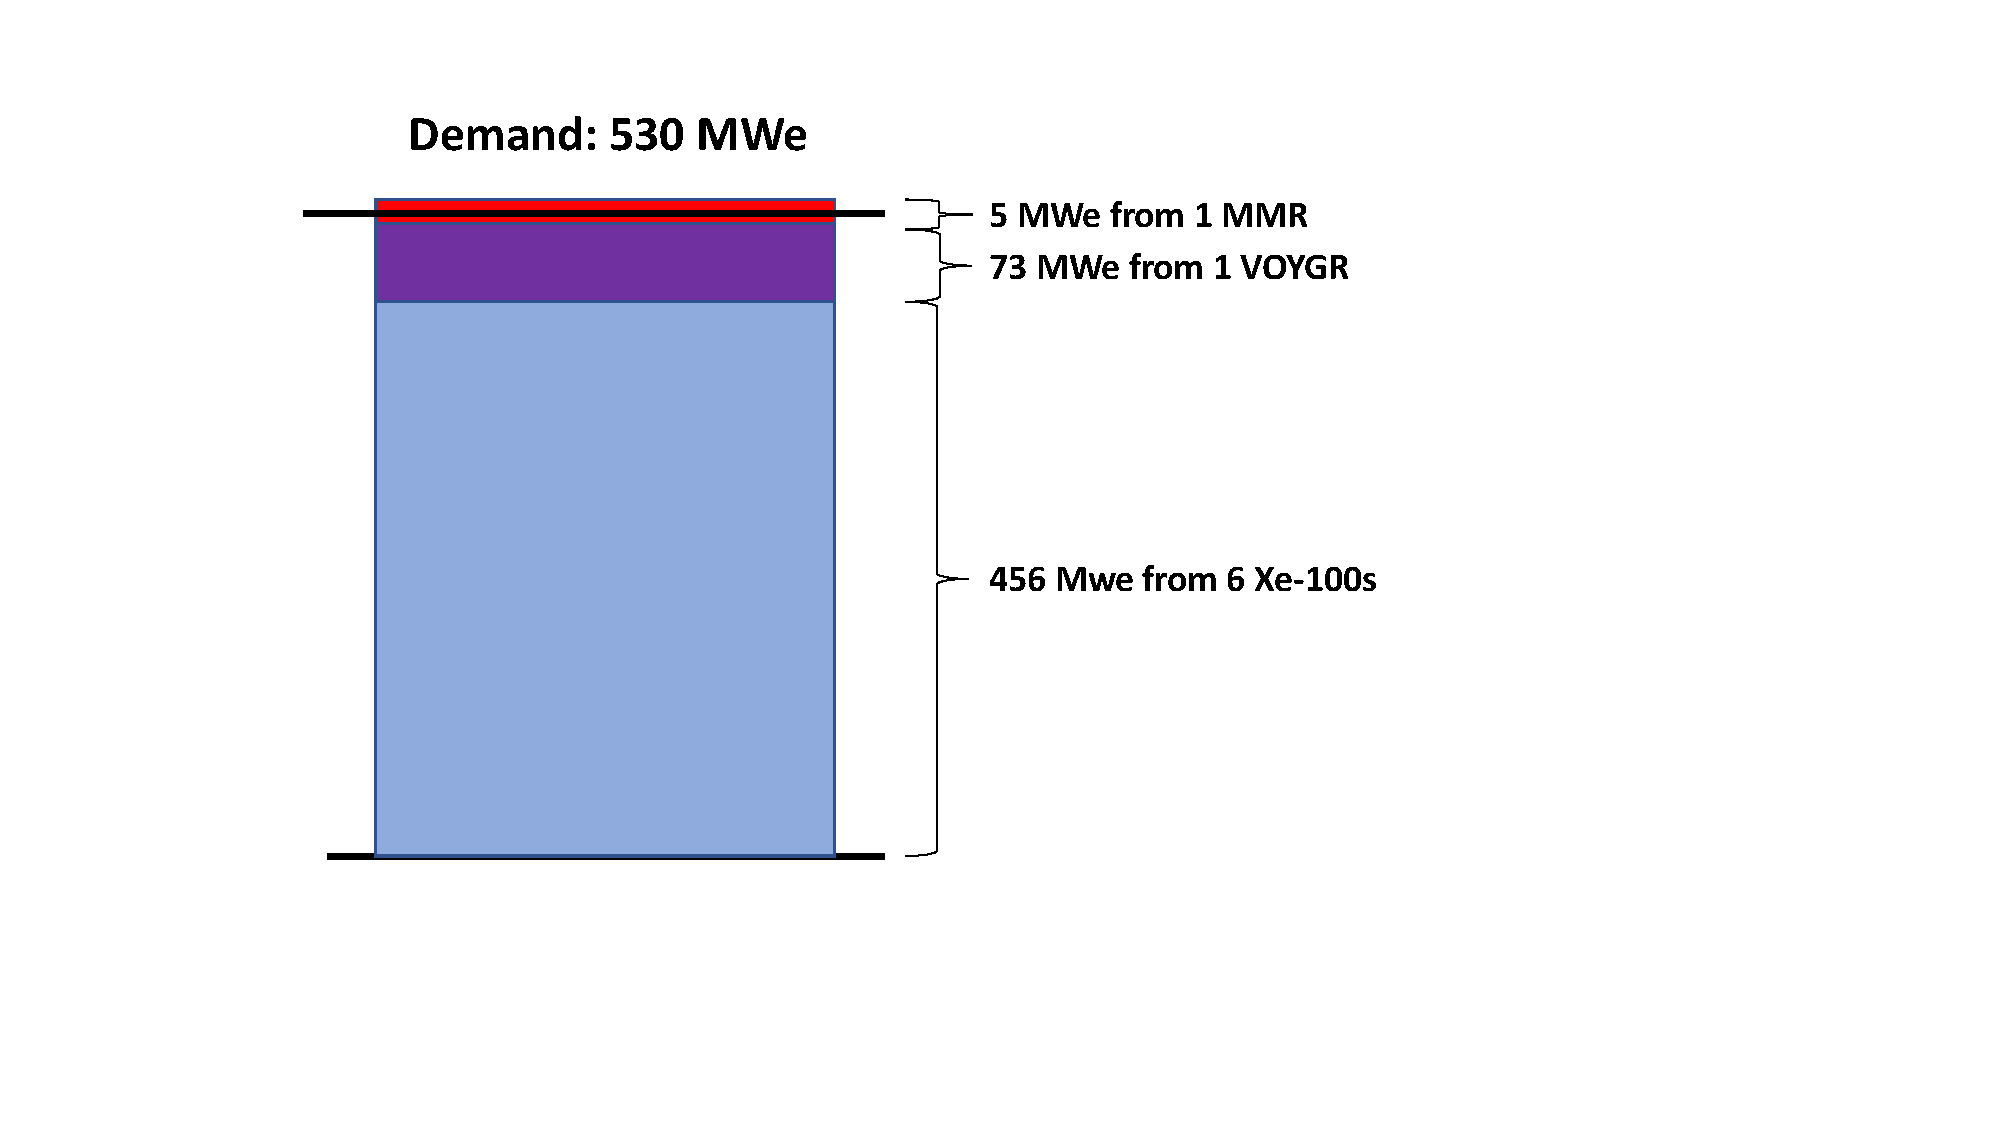
\includegraphics[scale=0.5, trim=0 100 90 0,clip]{Deployment_Scheme.pdf}
    \caption{Example of how advanced reactors are deployed in Scenario 7 
    to meet a theoretical demand of 530 MWe.}
    \label{fig:AR_deployment}
\end{figure}

This deployment strategy is used to deploy advanced reactors when there is
unmet demand in energy from the decommissioning of \glspl{LWR} or 
when the demand increases (such as in the 1\% growth scenarios). When 
there is unmet demand from the decommissioning of advanced reactors, the 
advanced reactors are redeployed on almost a one-to-one basis. A slightly
smaller number of advanced reactors may be redeployed if there is an 
oversupply of power greater than the power output of the reactor to be 
redeployed. 

\section{Recycling fuel cycle}\label{sec:recycle-methods}
Transition scenarios with a closed fuel cycle were created
to investigate how this type of \gls{NFC} affects the material requirements 
and how the recycling scheme impacts them. The scenarios investigated in 
this analysis vary by the energy demand of the scenario and the recycling 
scheme (Table \ref{tab:scenarios_recycle}). Energy demands vary 
between a no growth and a 1\% growth model, using the same 
demand curves as the once-through 
fuel cycle models. Variations in the recycling 
scheme include either a limited or a continuous recycle. Limited recycle 
scenarios assume that \gls{SNF} is recycled once and disposed of after a 
second pass through the reactor. Continuous recycling assumes that all 
\gls{SNF} is recycled an unlimited number of times until all fissile 
material has been used. Both recycling schemes were considered in the 
\acrfull{ES} \cite{wigeland_nuclear_2014}, which led to their inclusion 
in this work. Another distinction between some of the 
scenarios is if spent \gls{TRISO} fuel is recycled. Reprocessing \gls{TRISO}
faces many challenges and many of the technologies are at a low technology 
readiness level \cite{arm_plan_2022,kiegiel_management_2022}.
Therefore, by modeling scenarios that do and do not recycle 
\gls{TRISO} we can model more realistic scenarios in which \gls{TRISO} 
is not recycled and more academic scenarios in which all spent fuel is 
recycled. 

\begin{table}[ht]
    \centering
    \caption{Summary of the recycle fuel cycle transition scenarios.}
    \label{tab:scenarios_recycle}
    \begin{tabular}{l l l l}
            \hline
            Scenario number & Energy growth model & Recycle scheme & \gls{TRISO} recycled?\\
            \hline
            14 & No growth & Limited & Yes\\
            15 & No growth & Limited & No\\
            16 & No growth & Continuous & N/A \\
            17 & 1\% growth & Limited & Yes\\
            18 & 1\% growth & Limited & No\\
            19 & 1\% growth & Continuous & N/A \\
            \hline
    \end{tabular}
\end{table}

All of the scenarios with limited recycling model the transition from the 
current fleet of \glspl{LWR} to the X-energy Xe-100, the \gls{USNC} \gls{MMR}, 
and the NuScale VOYGR, the same as in scenarios 7 and 13. Therefore, 
the advanced reactor deployment schedules for these two scenarios are applied 
to the limited recycling scenarios for the appropriate energy growth model. 
This combination 
of reactors is considered for this step of the work, and not all of the 
combinations considered for the once-through scenarios, to limit the scope 
of the work but providing some comparison between the 
once-through and recycle transition scenarios. Because these scenarios 
use the same advanced reactor deployment schedule, the number of 
advanced reactors and the energy supplied are not examined in the 
results because they will be the same for each of these scenarios. Instead, 
the results of these scenarios will focus on the material requirements. 

For this work, the \glspl{LWR} and \gls{MMR} are modeled using the 
\Cycamore \texttt{Reactor} archetype. Each of these reactors use the 
fresh and spent fuel recipes that are used for the once-through scenarios. 
The Xe-100 and VOYGR are modeled using the DepleteReactor 
archetype from the OpenMCyclus library. The OpenMCyclus library was 
developed for this work to expand the capabilities of \Cyclus archetypes 
to dynamically modeling fuel depletion during a simulation. Section 
\ref{sec:openmcyclus} provides more details on how this archetype 
works and how it compares to the \Cycamore \texttt{Reactor} 
archetype. OpenMCyclus couples with the stand-alone depletion 
solver in OpenMC \cite{romano_depletion_2021}, thus, modeling a 
reactor using this archetype requires information about the refueling 
scheme for the reactor but also one-group cross section data to perform the 
depletion. 

For the VOYGR, we generated the one-group cross section data by using the 
built-in \gls{PWR} assembly model in OpenMC. We modified this model so 
that the Serpent \cite{leppanen_serpent_2014} 
and the Xe-100-like model described in Section 
\ref{sec:xe100_serpent_model} to generate the cross section data, then
post-processed the cross section data from Serpent to match the 
format required by OpenMC. For both reactors, we used the simplified 
depletion chain from OpenMC (referred to as the CASL chain) 
\cite{romano_depletion_2021}. Using this depletion chain results in  
adequate accuracy to the full depletion chain \cite{romano_depletion_2021}
and reduced run times compared with the full depletion chain.  

\subsection{Limited recycle scenarios}
Figure \ref{fig:limited_recycle_flow} shows the fuel cycle and material flows 
for the scenarios with limited recycling (Scenarios 14, 15, 17, and 18). 
In Scenarios 15 and 18 only the spent fuel from the 
VOYGRs is sent to the reprocessing facility, but in Scenarios 14 and 17, 
all spent fuel from the advanced reactors is sent to the 
reprocessing facility. Only the Xe-100 and VOYGRs receive \gls{MOX} fuel, 
but not the \glspl{MMR} to simplify the fuel cycle.

\begin{figure}
    \centering
    \begin{tikzpicture}[node distance=1.5cm]
        \node (mine) [facility, text width=1cm] {Uranium Mine};
        \node (enrichment) [facility, below of=mine]{Enrichment};
        \node (reactor) [facility, below of=enrichment]{LWR};
        \node (mmr) [transition, right of=reactor, xshift=1.5cm]{MMR};
        \node (xe100) [transition, right of=mmr, xshift=1.5cm]{Xe-100};
        \node (voygr) [transition, right of=xe100, xshift=1.5cm]{VOYGR};
        \node (wetstorage) [facility, below of=reactor, text width=1cm]{Cooling Pool};
        \node (drystorage) [facility, below of=wetstorage, text width=1.5cm]{Dry Storage};
        \node (cooling) [transition, below of=mmr, xshift=1.5cm, text width=1cm]{Cooling Pool};
        \node (sinkhlw) [facility, below of=drystorage, xshift=2.5cm, yshift=-1cm]{Repository};
        \node (sinkllw) [facility, left of=enrichment, xshift=-1.5cm, text width=1cm]{Tails Sink};
        \node (separation) [transition, below of=cooling, yshift=-1cm]{Separations};
        \node (mox_fab) [transition, below of=voygr,xshift=2cm, text width=1cm]{MOX Fuel Fab};
        \node (mox_cooling) [transition, below of=xe100, xshift=1.5cm, yshift=-1.5cm]{MOX Cooling};
        
        \draw [arrow] (mine) -- node[anchor=west]{Natural uranium} (enrichment);
        \draw [arrow] (enrichment) -- node[anchor=east]{Fresh UOX}(reactor);
        \draw [arrow] (enrichment) -- node[anchor=south]{Tails}(sinkllw);
        \draw [arrow] (enrichment) -| (mmr);
        \draw [arrow] (enrichment) -| node[anchor=south]{Fresh UOX}(xe100);
        \draw [arrow] (enrichment) -| (voygr);
        \draw [arrow] (reactor) -- node[anchor=east]{Spent UOX}(wetstorage);
        \draw [arrow] (wetstorage) -- node[anchor=east]{Cool Spent UOX}(drystorage);
        \draw [arrow] (drystorage) |- node[anchor=east]{Casked Spent UOX}(sinkhlw);
        \draw [arrow] (mmr) |- node[anchor=east]{Spent UOX}(cooling);
        \draw [arrow] (xe100) |- (cooling);
        \draw [arrow] (voygr) |- node[anchor=south]{Spent UOX}(cooling);
        \draw [arrow] (xe100) -| (mox_cooling);
        \draw [arrow] (voygr) -| node[anchor=south, text width=1cm, pos=0.25]{Spent MOX}(mox_cooling);
        \draw [arrow] (cooling) -- node[anchor=west, text width=1.5cm]{Cooled Spent UOX}(separation);
        \draw [arrow] (separation) -| node[anchor=south,text width=1.5cm, pos=0.4]{Separated fissile material}(mox_fab);
        \draw [arrow] (separation) -| node[anchor=south, text width=1.5cm]{Fission Products}(sinkhlw);
        \draw [arrow] (mine) -| node[anchor=south, pos=0.4]{Natural uranium} (mox_fab);
        \draw [arrow] (mox_cooling) |- node[anchor=south]{Cool Spent MOX}(sinkhlw);
        \draw [arrow] (mox_fab.east) - ++(5mm,0) |- node[anchor=south, pos=0.5, text width=1.5cm]{Fresh MOX}(voygr.east);
        %\draw [arrow] (mox_fab.east) -| ++(5mm,0) -| (xe100.north);
        \end{tikzpicture}
    \caption{Fuel cycle facilities and material flow between facilities for modeling the transition 
    to advanced reactors with a limited recycle fuel cycle. The separations facility
    is deployed in 2020, five years before the transition. Before 2020 a once-through 
    fuel cycle is used with the facilities in blue.}
    \label{fig:limited_recycle_flow}
\end{figure}

A separations facility is deployed 5 years before the transition 
begins (i.e. in January 2020), as this strategy is commonly used for modeling 
transitions with recycling \cite{passerini_systematic_2014,richards_application_2021}
to ensure that enough fuel can be separated and 
processed in time for use in advanced reactors. Although this is a 
non-physical time to begin recycling in the US, using this timeline ensures 
that there will be enough reprocessed fuel to fuel all of the advanced 
reactors, and one can observe the maximum benefit of recycling. Additionally 
by using this timeline, specifically ensuring that advanced reactors 
are deployed at the same time as when they are deployed in the once-through 
transition, provides an even comparison between these fuel cycle options.
Based on the timeline of the separations facility deployment, only the 
\gls{UNF} from the \glspl{LWR} that is leaves wet storage (i.e., the 
Cooling Pool facility in Figure \ref{fig:limited_recycle_flow}) after 
2020 is reprocessed. 

The separations facility separates out plutonium from the other 
materials in the fuel, emulating the aqueous reprocessing method although the 
chemistry is not explicitly modeled. The partitioning factor is 99\% for
plutonium, based on a conservative estimate of stated 
process loses for aqueous reprocessing \cite{herbst_6_2011} and the 
separation efficiency previously used in previous fuel cycle modeling 
\cite{wigeland_nuclear_2014,sunny_transition_2015}. The separated 
material from this facility is then sent to a \gls{MOX} fuel fabrication 
facility that produces \gls{MOX} with a pre-defined composition for the 
advanced reactors. To determine the plutonium fraction in the 
\gls{MOX} fuel, we calculated the plutonium equivalence of the $^{235}$U 
based on the cross section data generated for the Xe-100 and VOYGR. All 
plutonium in the \gls{MOX} is $^{239}$Pu, even though 
fabricated \gls{MOX} will have other plutonium isotopes present, as 
a simplifying assumption. Using this 
method helps ensure that the fuel used will allow the 
reactor to run for the same cycle time and have the same assembly mass 
despite the different properties of $^{235}$U and $^{239}$Pu.
The separated plutonium is the fissile stream for the \gls{MOX} 
fuel fabrication, and natural uranium from the mine is the filler 
materials. The separation step is modeled using the \Cycamore 
\texttt{Separations} archetype, and the \gls{MOX} fuel fabrication is modeled 
using the \Cycamore \texttt{Mixer} archetype. The \texttt{Mixer} archetype 
combines the separated plutonium and natural uranium material 
streams in the constant ratios required to produce the \gls{MOX} fuel
that corresponds to composition for each reactor. 

\subsection{Continuous recycle scenarios}
Figure \ref{fig:continuous_recycle_flow} shows the facilities and material 
flow for the continuous recycle fuel cycle (Scenarios 16 and 19). Continuous recycle 
requires a fast reactor, but all of the reactors considered in this 
work so far have a thermal neutron energy spectrum. Therefore, the advanced 
reactors used in the other scenarios are replaced with a \gls{SFR}. 
The fast reactor is modeled based on the PRISM design from 
\gls{GEH} in the \gls{UNF} Recycle mode \cite{triplett_prism:_2012}, because of 
the availability of open-source information to accurately model the design
and fuel compositions. Table \ref{tab:fast_rx} defines some of the 
design parameters of the \gls{SFR} in this work. The \gls{SFR} was modeled 
using the OpenMCyclus DepleteReactor archetype. 

\begin{figure}
    \centering
    \begin{tikzpicture}[node distance=1.5cm]
        \node (mine) [facility] {Uranium Mine};
        \node (enrichment) [facility, below of=mine]{Enrichment};
        \node (reactor) [facility, below of=enrichment]{LWR};
        \node (adv_reactor) [transition, right of=reactor, xshift=3cm]{Advanced Reactor};
        \node (wetstorage) [facility, below of=reactor]{Wet Storage};
        \node (drystorage) [facility, below of=wetstorage]{Dry Storage};
        \node (cooling) [transition, below of=adv_reactor]{Cooling Pool};
        \node (sinkhlw) [facility, below of=drystorage, xshift=2.5cm]{Repository};
        \node (sinkllw) [facility, left of=enrichment, xshift=-3cm]{Tails sink};
        \node (separation) [transition, below of=cooling]{Separations};
        \node (fuelfab) [transition, below of=adv_reactor,xshift=3cm]{Fuel Fab};
        \node (sfr) [transition, right of=adv_reactor, xshift=3.5cm]{Fast Reactor};

        \draw [arrow] (mine) -- node[anchor=east]{Natural U} (enrichment);
        \draw [arrow] (enrichment) -- node[anchor=east]{Enriched U}(reactor);
        \draw [arrow] (enrichment) -- node[anchor=south]{Tails}(sinkllw);
        \draw [arrow] (enrichment) -| node[anchor=west]{Fresh Fuel}(adv_reactor);
        \draw [arrow] (reactor) -- node[anchor=east]{Spent UOX}(wetstorage);
        \draw [arrow] (wetstorage) -- node[anchor=east]{Cool Spent UOX}(drystorage);
        \draw [arrow] (drystorage) |- node[anchor=east]{Casked Spent UOX}(sinkhlw);
        \draw [arrow] (adv_reactor) -- node[anchor=west]{Spent Fuel}(cooling);
        \draw [arrow] (cooling) -- node[anchor=west]{Cooled Spent Fuel}(separation);
        \draw [arrow] (separation) -| node[anchor=north, text width=1.5cm]{Separated fissile material}(fuelfab);
        \draw [arrow] (fuelfab) |- node[anchor=south, text width=1.5cm]{Reprocessed fuel}(sfr);
        \draw [arrow] (fuelfab) |- (adv_reactor);
        \draw [arrow] (separation) |- node[pos= 0.3, anchor=west, text width = 1.5cm]{Fission products}(sinkhlw);
        \draw [arrow] (wetstorage) -- node[sloped, anchor=south]{Cool Spent UOX}(separation);
        \draw [arrow] (sfr) |- node[anchor=west]{Waste}(sinkhlw);
        \draw [arrow] (mine) -| node[anchor=south]{Natural uranium}(sfr);

        \end{tikzpicture}
    \caption{Fuel cycle facilities and material flow between facilities for modeling the transition 
    to advanced reactors with a continuous recycle fuel cycle. Before 2020 a once-through 
    fuel cycle is used with the facilities in blue. Facilities in red are deployed 
    in 2025, and represent all of the facilities and material flows in red in 
    Figure \ref{fig:limited_recycle_flow}.}
    \label{fig:continuous_recycle_flow}
\end{figure}

\begin{table}
    \centering
    \begin{threeparttable}

    \caption{Fast reactor design specification.}
    \label{tab:fast_rx}
    \begin{tabular}{l l}
        \hline
        Design Criteria & PRISM \cite{triplett_prism:_2012,fichtlscherer_assessing_2019}\\
        \hline
        Reactor type & Sodium Fast Reactor\\
        Power Output (MWth) & 840 \\
        Capacity Factor & 90\%\tnote{1} \\
        Enrichment (wt\% fissile Pu) &  11.3/13.5\tnote{2}\\
        Cycle Length (yrs) & 1 \\
        Number of cycles &  4\\
        Fuel form &  Metallic \\
        Discharge fuel burnup (MWd/kg HM) & 87.51 \\
        Reactor Lifetime (yrs)&  60\\
        \hline
    \end{tabular}
    \begin{tablenotes}
        \item [1] Assumed value
        \item [2] The PRISM in UNF Recycle mode has two different drive fuel compositions,
                  which are averaged based on the number of each assembly type to determine 
                  the fresh fuel composition for this reactor.
    \end{tablenotes}
\end{threeparttable}
\end{table}

To generate the one-group cross section data needed for 
depletion we developed an OpenMC model of the PRISM reactor in 
an equilibrium state (shown in 
Figure \ref{fig:prism_model}). Information about the 
dimensions and core configuration of the reactor were found in 
\cite{triplett_prism:_2012,fichtlscherer_assessing_2019}. 
These sources also provided some 
information about the fresh fuel composition (the ``reprocessed 
fuel'' material in Figure \ref{fig:continuous_recycle_flow}), which 
we supplemented 
with the isotopic ratios defined for the S-PRISM reactor (a 1000 MWth
\gls{SFR} of a similar design) in \cite{sumner_effects_2011}.
We then used the transport-coupled depletion solver in OpenMC to 
obtain compositions for each fuel batch at the beginning of cycle 
in this reactor. After revising the model to include each of the 
batch beginning of cycle compositions in the placements given 
in \cite{fichtlscherer_assessing_2019}, we ran the model 
through OpenMC again to obtain the one-group cross section data 
for this core in an equilibrium state. We calculated
the \gls{HALEU} composition required for this fuel cycle based on the
one-group cross section data and plutonium equivalence of 
uranium in this system.

\begin{figure}[h!]
    \centering
    \begin{subfigure}[b]{0.48\textwidth}
        \centering
        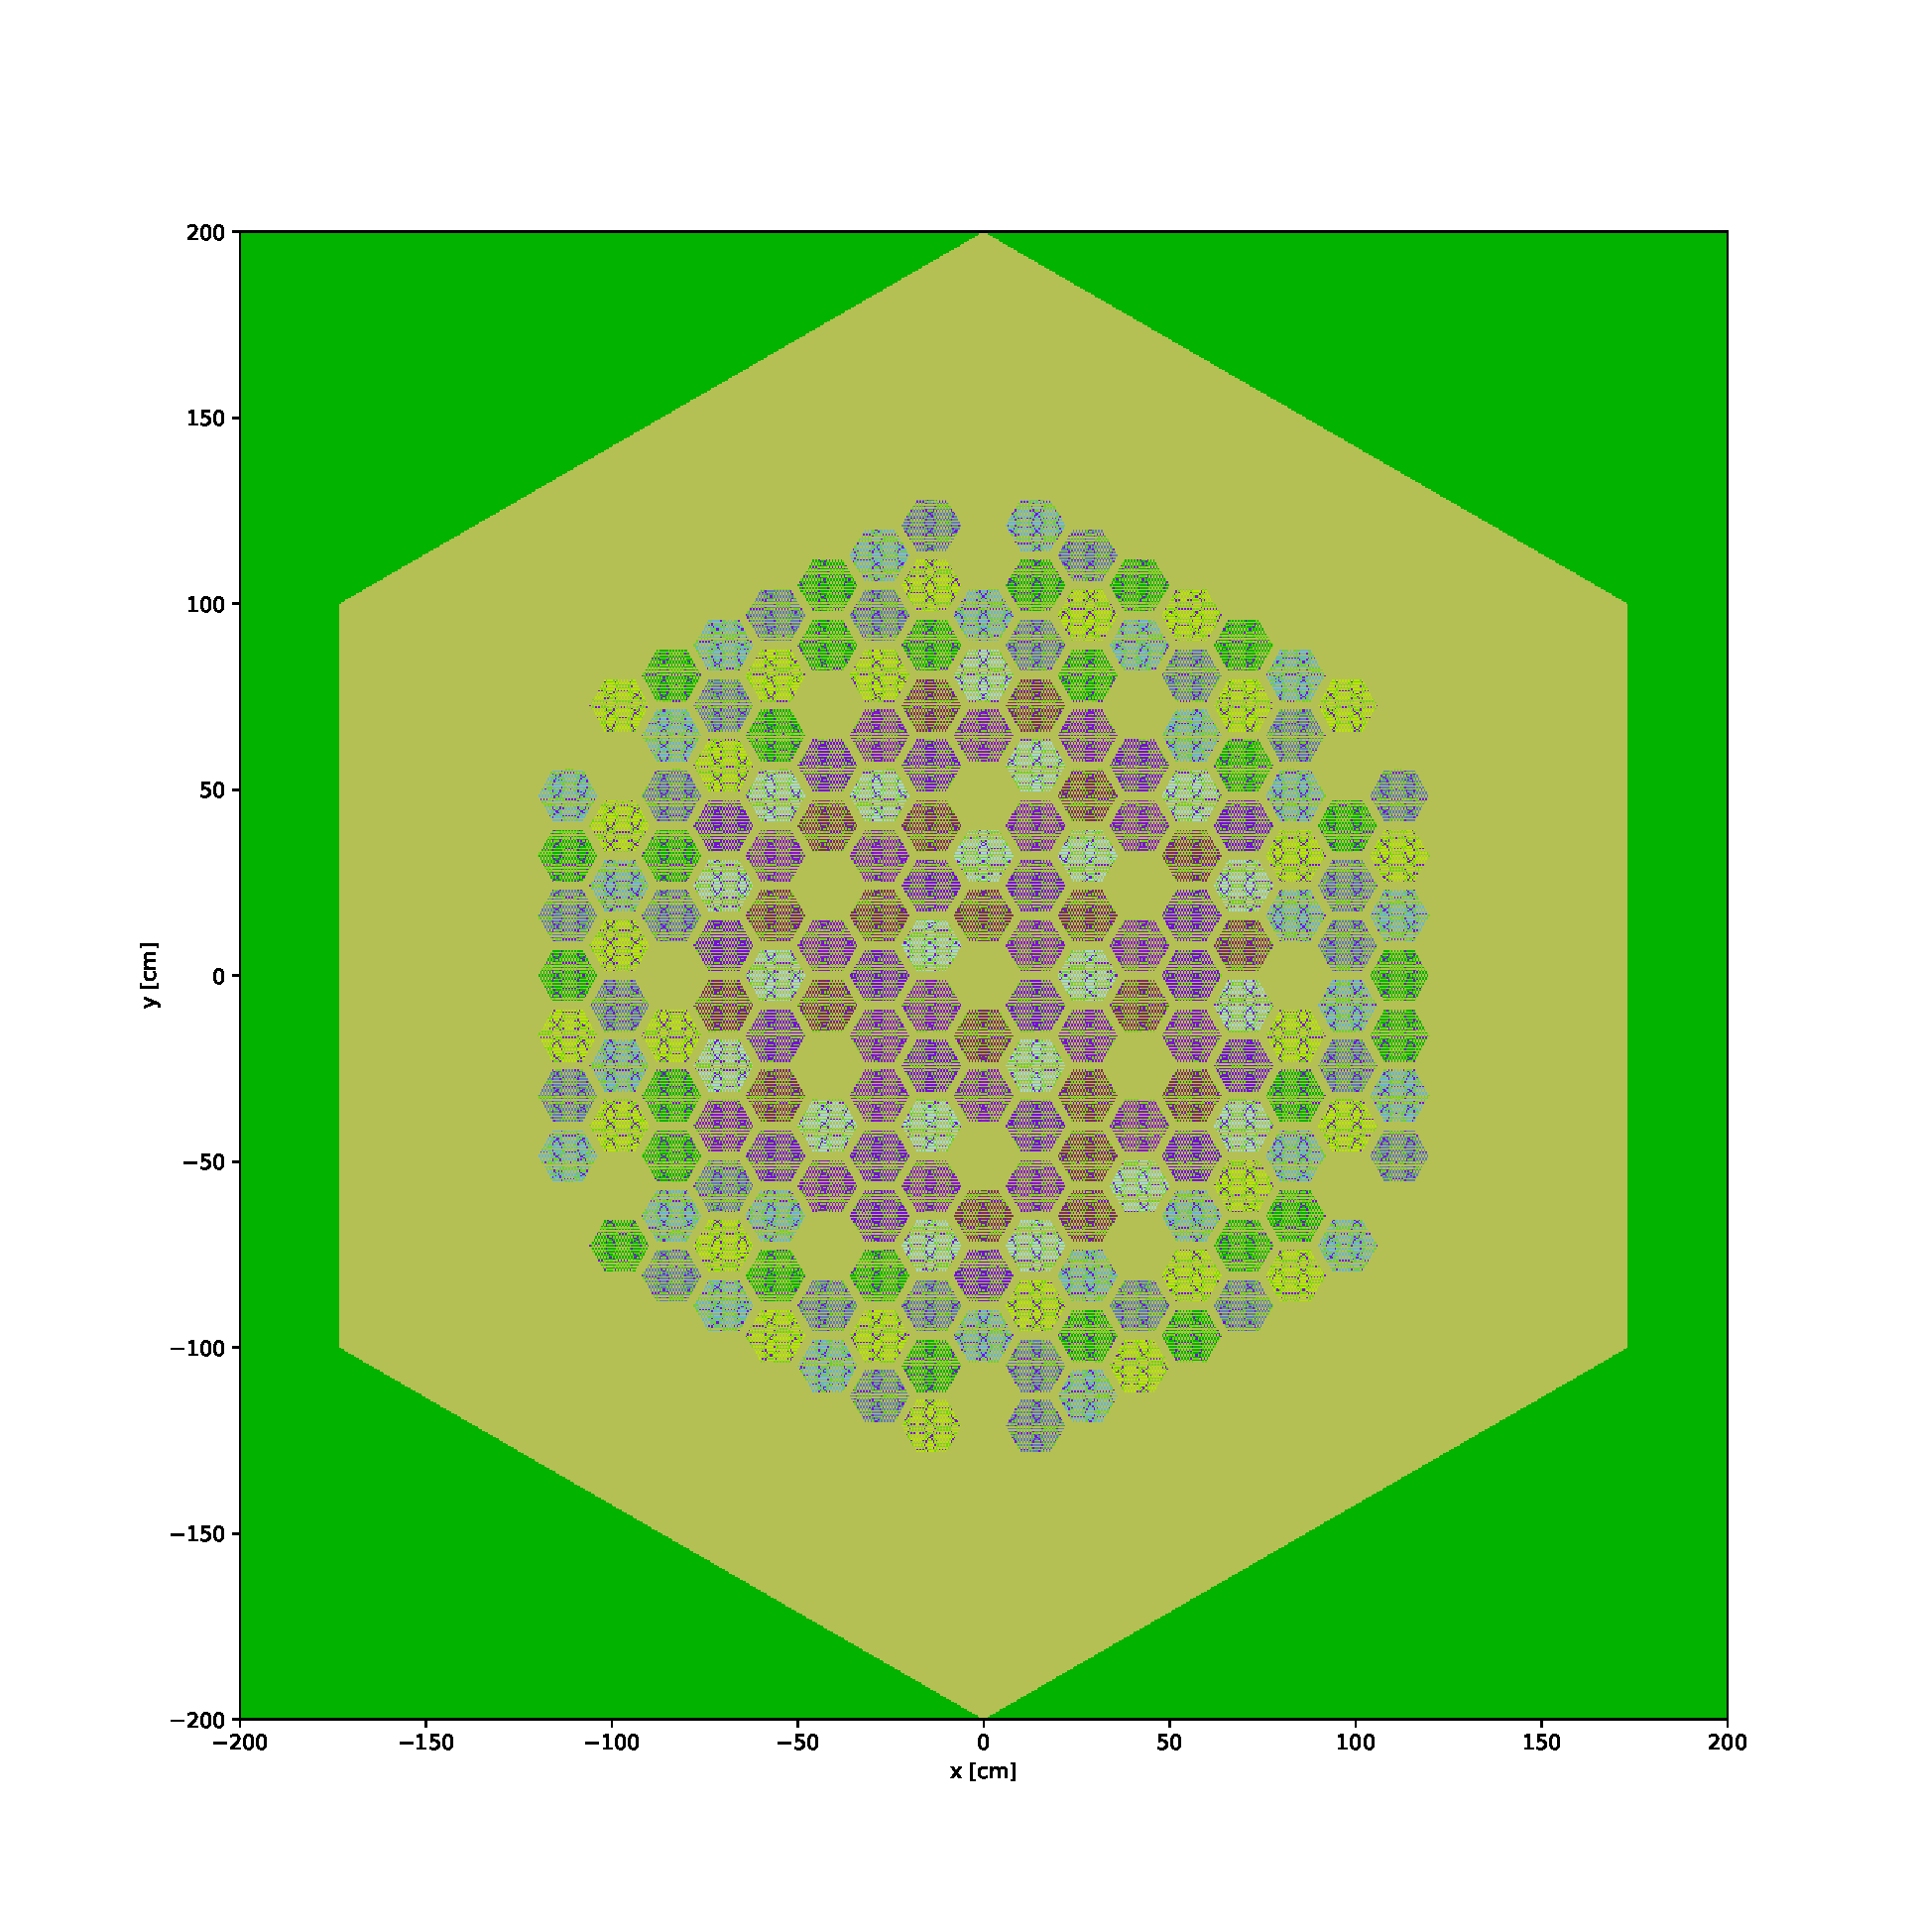
\includegraphics[width=\textwidth]{sfr_eq_core.pdf}
        \caption{Radial view of the entire PRISM model.}
        \label{fig:prism_lattice}
    \end{subfigure}
    \hfill
    \begin{subfigure}[b]{0.48\textwidth}
        \centering
        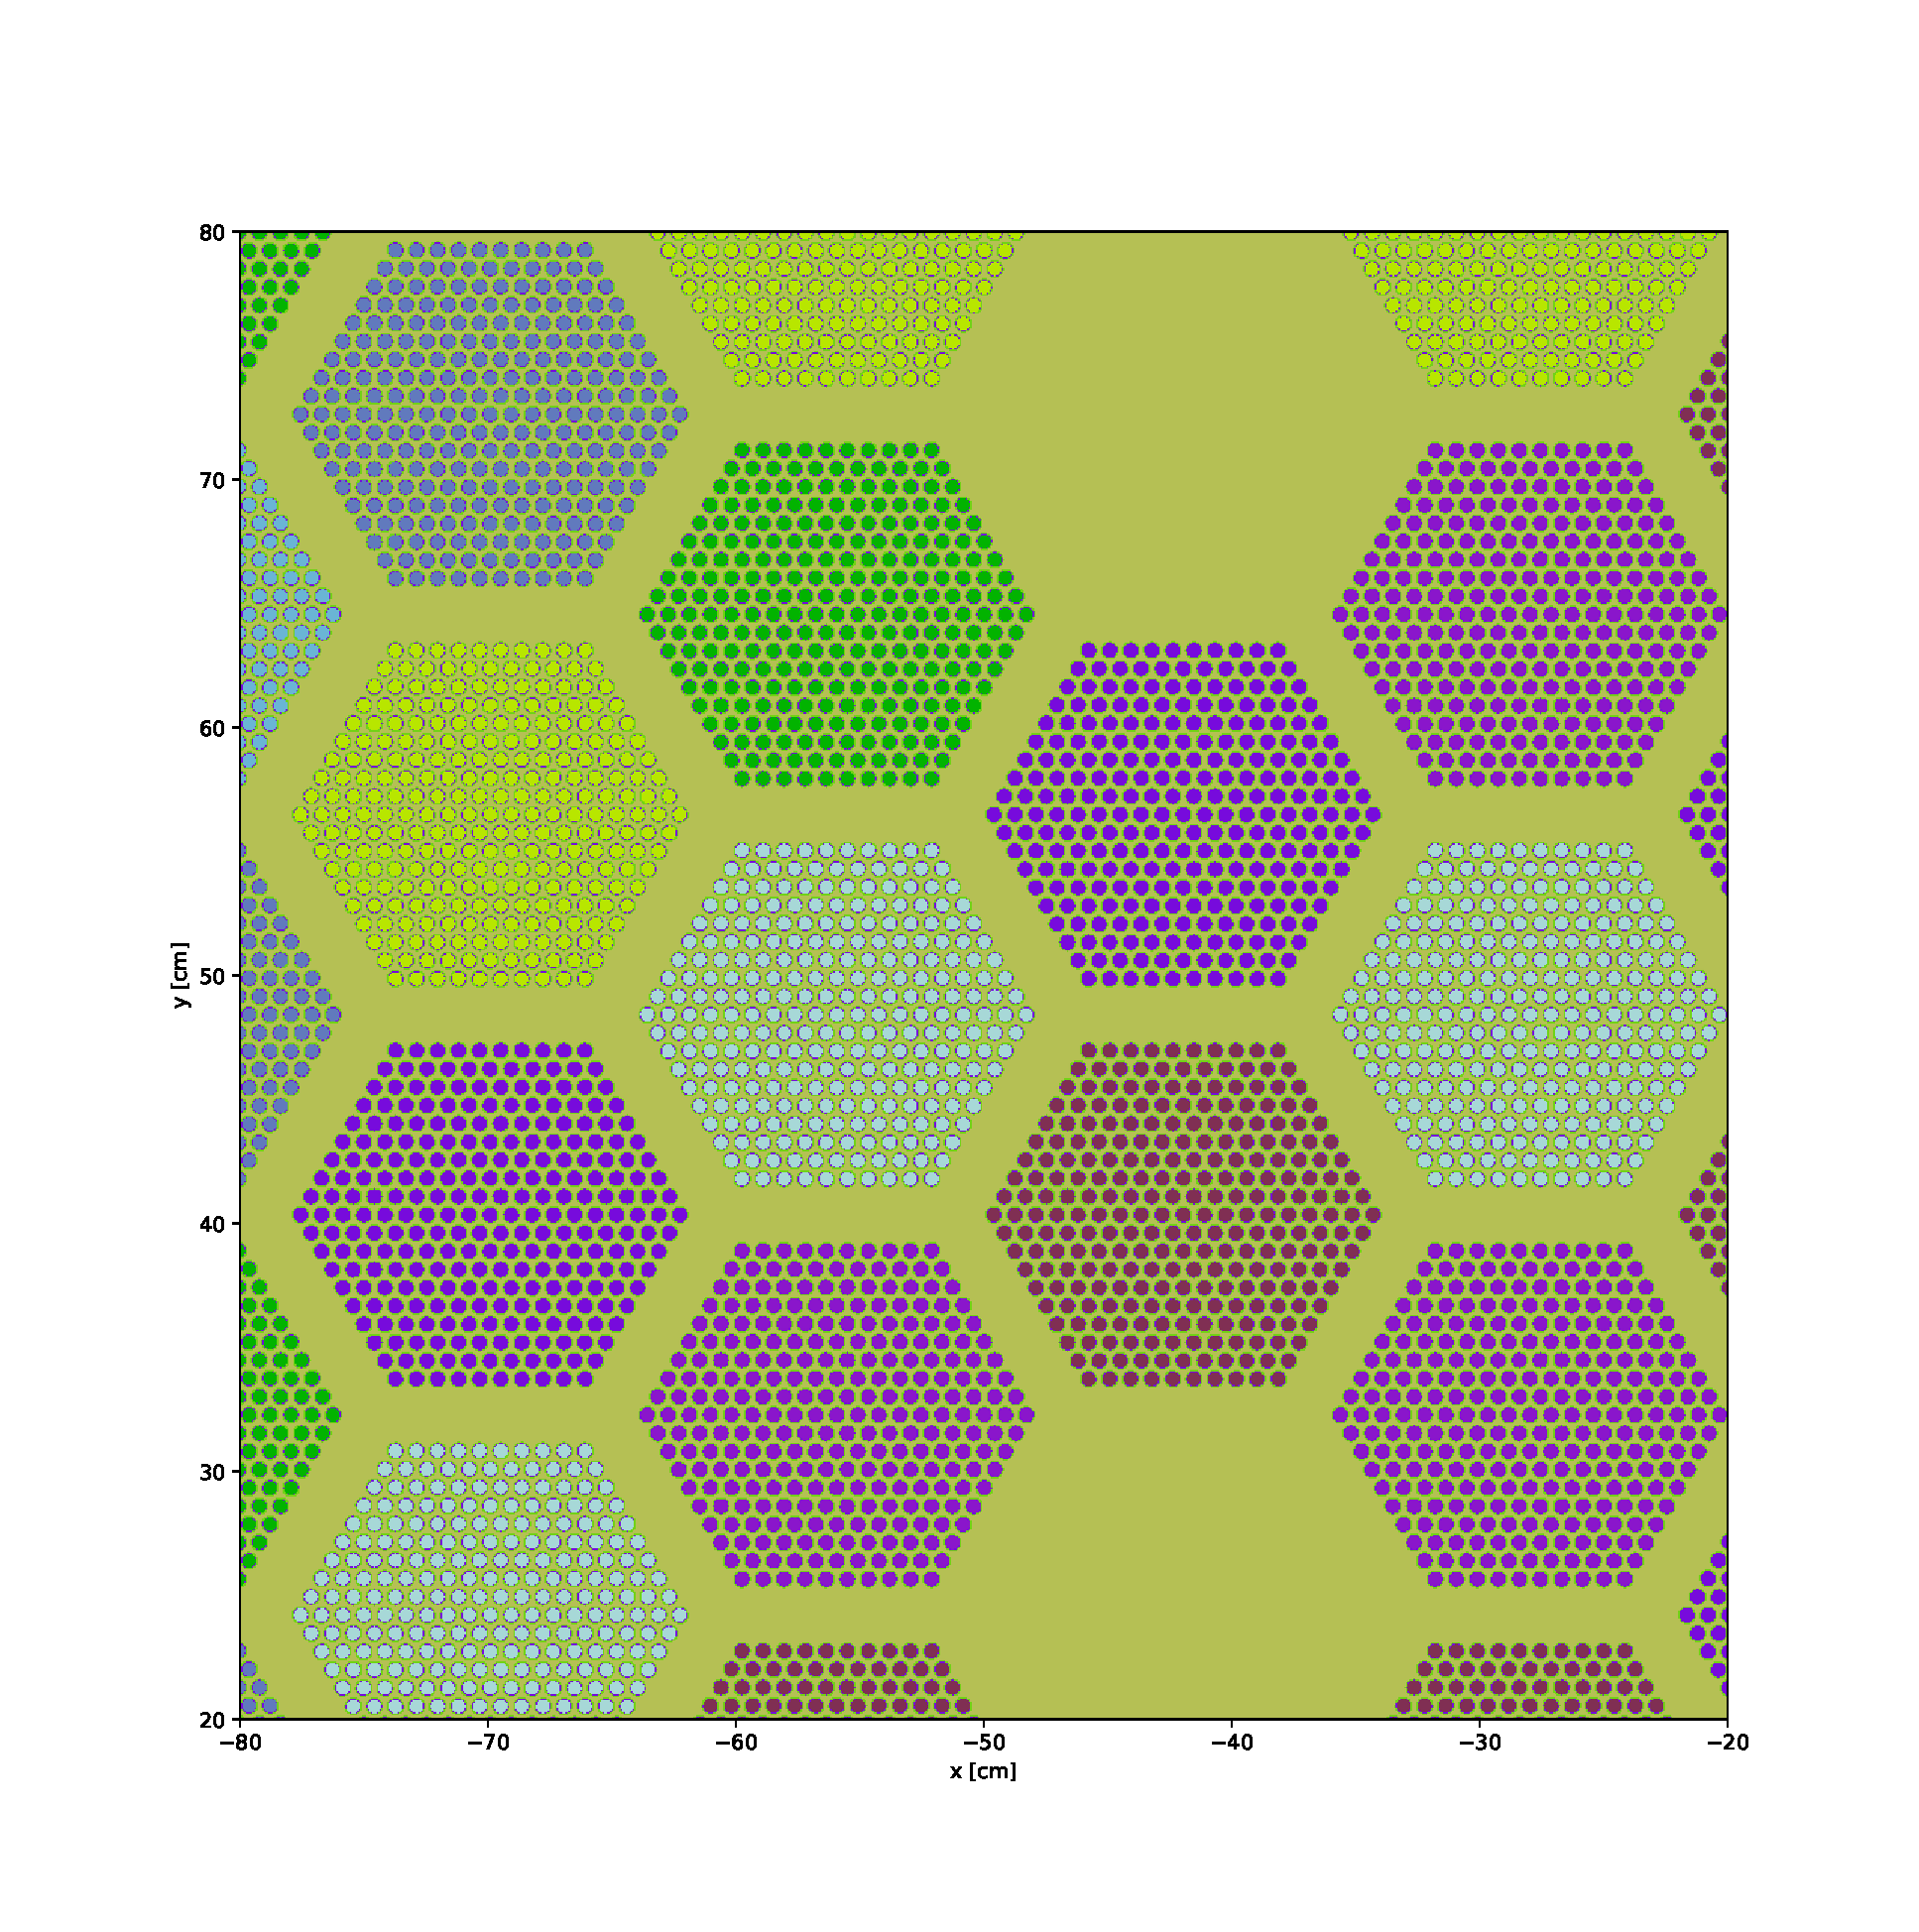
\includegraphics[width=\textwidth]{sfr_eq_core_zoom.pdf}
        \caption{Detailed view of the assembly lattice for each 
        fuel type.}
        \label{fig:prism_lattice_zoom}
    \end{subfigure}
    \hfill            
    \caption{Full and zoomed in OpenMC models of the PRISM reactor, based 
    on information in \textbf{citations}. The gold material is the 
    sodium coolant, the purple is the inner fuel assemblies, and the 
    light green is the outer fuel assemblies. }
    \label{fig:prism_model}
\end{figure}

To support using reprocessed fuel in the fast reactor, 
the separations facility is deployed in 2020, similar to in the 
limited recycling scenarios, and uranium and transuranic elements 
(neptunium, plutonium, americium) are separated out from 
the spent fuel with 99\% efficiency. If not enough reprocessed fuel is 
available to support the fast reactor fleet, then \gls{HALEU} is supplied
to fuel the reactors, but the reactors have a preference for reprocessed 
fuel over \gls{HALEU}. We calculated the fuel mass using Eq. \ref{eq:fuel_mass},
and divided as needed for the mass of each assembly in the core. 
We also calculated the deployment scheme for this reactor using the 
same methodology described in Section \ref{sec:reactor_methods}, based on 
the applicable demand curve (no growth for Scenario 16 and 1\% growth 
for Scenario 19), the power output of the \gls{SFR}, and the capacity 
factor of the \gls{SFR}.

\section{Calculation of results} \label{sec:results_calc}
The results of the transition scenarios modeled include the energy generated, 
the number of advanced reactors deployed, the mass of enriched uranium, 
mass of feed uranium, \gls{SWU} capacity required to produce the enriched 
uranium, and the \gls{SNF} discharged from the reactors. Each of these results 
are obtained from the \Cyclus output file of the simulation. 

The energy generated in each scenario is calculated and  
reported by \Cyclus. Each reactor facility produces a 
commodity called ``power'', and the total output of each reactor facility 
is reported at each time step that they produce it. 
\Cyclus reports the time step that each facility in the simulation enters 
(commissions) and exits (decommissions) the simulation. Based on 
this information the total number of each type of reactor is 
determined. 

The other results in this work are calculated based on commodity 
transactions to and from the facilities. The mass of enriched 
uranium is the mass of fuel traded between the enrichment facility and 
the reactors, multiplied by the mass fraction of uranium in the fuel 
form. Multiplying by the mass fraction of uranium means that the other 
fuel components are not included in this mass and the reported mass is 
the product produced by an enrichment facility, $P$ in Eq. 
\ref{eq:enrichment}. This methodology does not account for any 
losses from fuel fabrication.

The feed uranium masses and \gls{SWU} capacity are calculated 
based on the mass of enriched uranium traded to the reactors, using 
Eq. \ref{eq:enrichment}. The natural uranium traded to the enrichment 
facility is not used for this result because the enrichment facility 
does not have a 
specified limit on the amount of feed material it can store. Therefore, 
the enrichment facility continuously requests and receives feed 
uranium from the uranium mine without consideration for how much it needs 
to produce the enriched uranium for the reactors. This work does not 
place a limit on the enrichment facility capacity to ensure that the 
reactors are fully fueled and prevent other facility limits to 
influence the reported material demands. 

Finally, in the once through scenarios the mass of \gls{SNF} generated is 
the mass of spent fuel that is 
traded from the reactor facilities to the cooling pools. This mass is the 
entire fuel form, not just the uranium or heavy metal mass in the spent 
fuel, because the entire fuel form must be considered when determining 
disposal needs and options. In the recycling scenarios, the spent fuel 
mass is the mass traded from separations and \gls{MOX} cooling facilities 
to the repository. This change in the calculation of spent fuel mass 
in the recycling scenarios is because not all of the material discharged 
from the reactors is disposed of in these scenarios, and the inclusion of 
the waste from reprocessing is captured in this metric.

\section{OpenMCyclus}\label{sec:openmcyclus}
OpenMCyclus is an archetype library that holds the DepleteReactor 
archetype, and is publicly available \cite{bachmann_openmcyclus_2023}. 
Currently, OpenMCyclus only holds this one archetype, so 
the two terms are used synonymously across this work. OpenMCyclus couples 
\Cyclus with the stand-alone depletion solver in OpenMC 
\cite{romano_depletion_2021} to provide 
dynamic updates of spent fuel composition during a fuel cycle simulation.
This coupling arose because 
of the open-source nature of OpenMC and its rich Python \gls{API}. 
The open-source nature of OpenMC complements the open-source nature 
of \Cyclus to prevent creating additional obstacles in using the archetype. 
Additionally, the Python \gls{API} of OpenMC complements the Python 
\gls{API} of \Cyclus, aiding in the development of the archetype. 
There are two primary components to OpenMCyclus: fuel depletion and 
transmutation and the material handling. 

\subsection{Fuel depletion and transmutation} \label{sec:transmute}
OpenMCyclus performs fuel depletion through  
the depletion solver in OpenMC, which solves a system 
of first-order ODEs that describes 
the rate of change of each nuclide as a function of production and loss 
mechanisms \cite{romano_depletion_2021}. OpenMC applies a \gls{CRAM} solver 
and multiple time integration methods to solve the system of equations, which 
has been shown to have good agreement with the depletion solver in Serpent 
\cite{romano_depletion_2021}. OpenMC provides this capability in two primary 
forms: transport dependent and transport independent solvers. To simplify 
the information needed and reduce run times, OpenMCyclus uses the transport 
independent solver through the \texttt{IndependentOperator} class of the 
\texttt{openmc.deplete} module. 

Using this class requires users to provide information including 
one-group microscopic cross section data, depletion chain data, the 
number of depletion steps, 
power level, and material compositions for the fuel. The multi-group 
cross section data must be provided by the user through a ``.csv'' file by 
specifying a path to the file, assumed to be titled ``micro\_xs.csv'' by the 
archetype. Users can obtain this data by running a transport calculation 
of the desired reactor geometry using OpenMC or another transport solver. 
The depletion chain data is an ``.xml'' file that is assumed to be in the 
same directory as the cross section data, under a filename that is specified 
by the user.
The depletion steps are 30 days each (corresponding to 1 month), 
with one depletion step for each month of the operating cycle, as defined by 
the user. The power level is defined by the user, and is converted from 
MW to W (units assumed by \Cyclus to units assumed by OpenMC). Each of these 
variables (depletion chain data file name, path to the cross section data and 
depletion chain data, the number of depletion steps, and the power level) are 
defined by the user through the \Cyclus input file then passed from the archetype 
to OpenMC. 

There are two different material definitions when using OpenMCyclus:
the fresh fuel composition and the OpenMC materials. The fresh fuel 
compositions are defined as a recipe in the \Cyclus input file. 
The OpenMC materials are passed to OpenMC for depletion, and are 
located in an ``.xml'' file 
(assumed to be in the same directory as the cross section and depletion 
chain data, and assumed to be titled ``materials.xml''). Information in 
this file includes the material ID, material name, material volume, material 
density, and the material composition. The information is 
read in by \Cyclus and the compositions are updated by the archetype to 
contain the composition of each assembly in the reactor when depletion is 
performed. The updated information in is then passed to
OpenMC for depletion. 

To account for multiple batches of fuel in the core, all of the assemblies 
are depleted and have their compositions updated 
at the end of each cycle, with the depletion time equaling one cycle 
length. This methodology differs from the \Cycamore 
\texttt{Reactor} archetype, which transmutes the composition of only the 
number of 
assemblies in a batch, and immediately changes the composition from that 
of the fresh fuel to that of spent fuel at the end of each cycle before the 
assemblies are discharged. Therefore, by accounting for 
changes in fresh fuel composition (e.g., UOX to MOX) and multiple 
batches in a core, OpenMCyclus is expected to be more sensitive to 
changes in spent fuel composition than the \Cycamore Reactor archetype. 
Additionally, the \Cycamore Reactor assumes that all spent fuel has the 
same composition, so even assemblies that are discharged after only one 
cycle have the same composition as those that are discharged after the
Additionally, when a reactor facility is decommissioned, the default behavior 
of the \Cycamore \texttt{Reactor} archetype is to transmute only half of the 
assemblies in the core, while the OpenMCyclus archetype transmutes all of 
the assemblies. This setting in the \Cycamore \texttt{Reactor} 
(\texttt{decom\_transmute\_all}) can be toggled to \texttt{True} so that 
both archetypes have the same behavior.

One known limitation of the depletion methodology in this archetype 
is that the cross section data does not get updated as the 
fuel compositions change. While this affects the accuracy of the 
spent fuel compositions, this methodology was chosen to provide 
a balance between fuel composition accuracy and computation 
resources to run a simulation with this archetype. 

\subsection{Material handling}
The material handling of the OpenMCyclus DepleteReactor archetype 
includes how material is transferred within different inventories 
in the archetype, how the archetype interacts with the \gls{DRE}, 
and how these interactions are recorded to the database. 

The DepleteReactor has three different material inventories that 
are internal to the archetype: ``fresh fuel'', ``core'', and ``spent 
fuel''. Each of these inventories are 
\texttt{cyclus.typesystem.ResBufMaterialInv} objects, which means that 
the material objects (i.e., fuel) can be moved between the different 
inventories as needed, and each inventory has a defined capacity. Movements 
between these inventories are not recorded to the database. The fresh 
fuel inventory represents extra fuel that is kept on site at the 
facility. The core inventory represents the fuel in the core 
and used for operating the reactor. The spent fuel inventory 
represents fuel that is finished in the core, and has been fully 
transmuted to the spent fuel composition. Material requests that 
are traded into the archetype can be placed in the fresh fuel 
or core inventories, based on the capacities of each. The 
material in the spent fuel inventory is used to generate bids 
for requests, and is traded away to other facilities when the bids 
are matched with a request by the \gls{DRE}. 

The frequency of material movement between these inventories and 
the timing of requests and bids in the \gls{DRE} are based on 
the user-defined cycle length and refuel time state variables. 
A reactor agent (a deployed prototype) requests enough fuel assemblies 
to fill the fresh fuel and core inventories.
Each fuel assembly to fill the fresh fuel and core inventories 
is a separate request, with each request 
being exclusive (i.e., partial fulfillment of the request by another 
agent is not allowed). If multiple commodities can meet a request for 
an assembly (e.g., UOX or MOX assemblies), then all of the possible 
commodities are requested through mutual requests based on user-defined 
preferences for each commodity. Materials are requested in quantities 
to match the user-defined assembly mass size. Information about the 
materials is recorded to the output database, including the 
commodity name, material mass, sending prototype, and the receiving 
prototype. If the agent 
receives enough fuel and the core inventory is filled, then the 
agent begins its operating cycle. During the operating cycle, the 
reactor is recorded as producing the user-defined power each time step 
of the cycle, and will only request more fuel assemblies if the 
fresh fuel inventory is not filled. At the end of the operating 
cycle, the fuel in the core is transmuted as described in Section 
\ref{sec:transmute}, and one batch of fuel (a user-defined state variable)
is discharged from the core inventory to the spent fuel inventory. 
If there is any fuel in the fresh fuel inventory, then it is 
loaded into the core. Then more fuel for the fresh fuel and the 
core inventories are requested from other facilities, and the 
materials in the spent fuel inventory are traded away if requested 
by other facilities. Before starting the next operating cycle, the 
facility experiences a refueling period, that lasts as long as the 
user-defined state variable. During this period, the facility does 
not produce any power. If the core is not full and within the operating 
cycle, then it does not produce any power. After the refueling period 
ends, the facility enters back into the operating cycle and repeats 
this process until it is retired or until the simulation ends. 

If the facility reaches the end of its lifetime during a simulation, 
all of the fuel in 
the core is transmuted one final time and all of the 
assemblies are discharged from the core to the spent fuel
inventory. If any assemblies in the fresh fuel inventory, then 
they are also moved to the spent fuel inventory to be traded 
away to other facilities. Once the core and spent fuel are 
both empty, the facility is decommissioned and exits the simulation.

\subsection{Comparison with \Cycamore Reactor}
To verify the results from OpenMCyclus, we created a sample fuel cycle 
scenario to model with the \Cycamore Reactor archetype and the 
OpenMCyclus DepleteReactor archetype. All of the code used to define the 
scenarios, generate data, and the analysis are publicly available 
\cite{bachmann_openmcyclus_2023}. The fuel cycle is 
shown in Figure 
\ref{fig:comparison}. Each of the non-reactor facilities are defined 
using archetypes in the \Cycamore library, with the \Cycamore \texttt{Mixer}
defining the ``MOX Fuel Fab'' agent. The \texttt{Mixer} agent takes in multiple 
material streams and combines them in a user-defined ratio to produce 
a final output stream. 

\begin{figure}
    \centering
    \begin{tikzpicture}[node distance=1.5cm]
        \node (mine) [facility] {Uranium Mine};
        \node (enrichment) [facility, below of=mine]{Enrichment};
        \node (reactor) [facility, below of=enrichment]{Reactor};
        \node (sinkhlw) [facility, below of=reactor, xshift=2.5cm, yshift=-1cm]{Repository};
        \node (separation) [facility, right of=reactor, xshift=2.5cm]{Separations};
        \node (mox_fab) [facility, above of=separation, yshift=0.8cm]{MOX Fuel Fab};
        
        \draw [arrow] (mine) -- node[anchor=east]{Natural uranium} (enrichment);
        \draw [arrow] (enrichment) -- node[anchor=east]{Fresh UOX}(reactor);
        \draw [arrow] (reactor) -- node[anchor=north]{Spent UOX}(separation);
        %\draw [arrow] (cooling) -- node[anchor=west, text width=1.5cm]{Cooled Spent UOX}(separation);
        \draw [arrow] (separation) -- node[anchor=west]{Separated plutonium}(mox_fab);
        \draw [arrow] (separation) |- node[anchor=west, pos=0.3]{Fission Products}(sinkhlw);
        \draw [arrow] (mine) -| node[anchor=south, pos=0.4]{Natural uranium} (mox_fab);
        \draw [arrow] (reactor) |- node[anchor=east, pos=0.3]{Spent MOX} (sinkhlw);
        \draw [arrow] (mox_fab) -- node[anchor=south, sloped]{Fresh MOX} (reactor);
        %\draw [arrow] (mox_fab.east) -| ++(5mm,0) -| (xe100.north);
        \end{tikzpicture}
    \caption{Fuel cycle facilities and material flow between facilities for the 
    sample fuel cycle scenarios used to compare the results of the \Cycamore Reactor 
    and OpenMCyclus DepleteReactor archetypes. }
    \label{fig:comparison}
\end{figure}

The entire simulation is 200 months. Reactors are deployed using the 
\Cycamore \texttt{DeployInst} institution archetype: 2 at time step 1, 
1 at time step 
50, 1 at time step 100, and 1 at time step 150. The reactors have a lifetime 
of 60 time steps, cycle length of 12 time steps, refueling length of 1 
time step, three batches per core, one assembly per batch, a power output of 
195 W, and an assembly size of 0.00602 kg. The reactors prefer MOX over UOX. 
 
To obtain a spent fuel composition for the \Cycamore \texttt{Reactor} 
archetype and cross section data for the DepleteReactor archetype, we 
used the pin cell example model in OpenMC \cite{noauthor_modeling_nodate}. 
Using this 
small model is a simplifying assumption about the size of the reactors, 
and led to the small power level and assembly mass of the prototypes. 
We used this model in OpenMC to generate the one-group cross 
section data required to define the \texttt{IndependentOperator} class 
in OpenMC. Using this cross section data, we depleted the pin cell 
model using OpenMC to obtain the spent UOX and 
spent MOX compositions, with the depletion modeling the entire time that 
an assembly would be in the the core (i.e., 36 months straight). 
These compositions were then converted into recipes for use in 
\Cyclus.
The one-group cross section data from OpenMC was then used to run 
OpenMCyclus, ensuring that the same data is used for both archetypes.  

We ran the scenario with the \Cycamore \texttt{Reactor} archetype twice, 
toggling the \texttt{decom\_transmute\_all} setting between \texttt{True}
and \texttt{False}. Toggling this setting allows us to explore how the 
different possible methodologies to handle the fuel upon a facility 
decommissioning in the \Cycamore \texttt{Reactor} affects the results of 
the simulation and provide a more comprehensive comparison between the 
two archetypes. We compared the archetypes based on the energy generated 
by the reactor prototypes and the transactions of fresh fuel, spent fuel, 
and separated plutonium. 

\subsubsection{Comparison results}
Comparing the energy provided from the different reactor archetypes is 
important because many 
fuel cycle scenarios are designed based on deploying reactors to meet a 
specific power demand. Therefore, ensuring that the DepleteReactor 
will produce the correct amount of power at the correct times 
supports its use for modeling fuel cycle transitions. 

Figure \ref{fig:comparison_power} shows the power provided from the
reactor prototypes when using each archetype.
There is perfect agreement between the archetypes, even with the different 
settings for the \Cycamore \texttt{Reactor}. At the start of the scenario, 
the prototypes produce 390 W of power, because two reactors are 
deployed. When the third reactor is deployed at time step 50, 
the power provided increases to 585 W. When there is only one  
reactor deployed (e.g., between time steps 63-99) 195 W of power 
are produced. Every 13th time step after a reactor facility deploys, 
the facility produced 0 W of power, signifying that it is refueling.
All of these results match expectations. 

\begin{figure}[ht]
    \centering 
    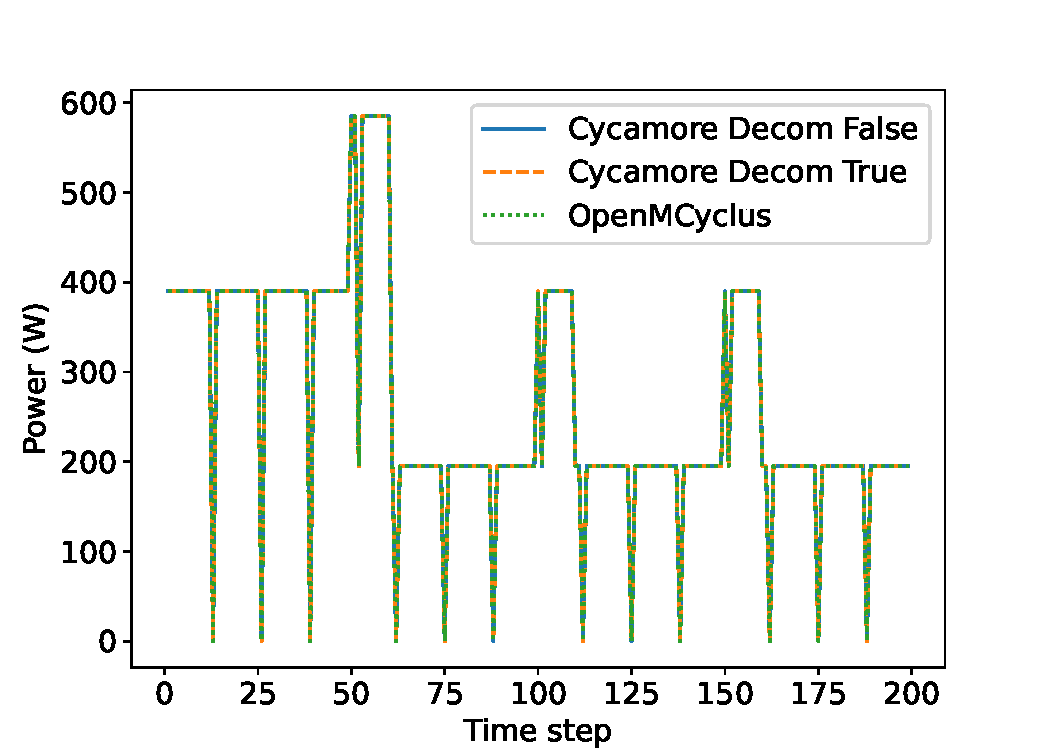
\includegraphics[scale=0.9]{comparison_energy.pdf}
    \caption{Comparison of power provided from reactor prototypes 
    when comparing the \Cycamore \texttt{Reactor} and OpenMCyclus 
    DepleteReactor archetypes.}
    \label{fig:comparison_power}
\end{figure}

Figure \ref{fig:comparison_fuel} shows the transactions of fresh UOX 
and fresh MOX fuel to the facilities when each archetype is used. There are 
differences between the archetypes in when they receive each fuel type. 
However, the total amount of fuel and when the fuel is received is in 
perfect agreement between all three scenarios. At each time step that 
a reactor facility is commissioned, a full core's worth of fuel (i.e., 
three assemblies) are sent to the reactor. The reactors also receive fuel 
at the correct intervals for refueling (every thirteen months or twelve 
after deployment because of the lack of refueling period). The differences 
that arise between the archetypes is in how much of each fuel commodity 
is received at each time step. Because the \gls{MOX} fuel is preferred 
over the \gls{UOX} fuel, the supply of plutonium available to create the 
\gls{MOX} fuel is the driving factor of this difference and the primary 
difference between these scenarios. 

\begin{figure}[ht!]
    \centering
    \begin{subfigure}[b]{0.48\textwidth}
        \centering
        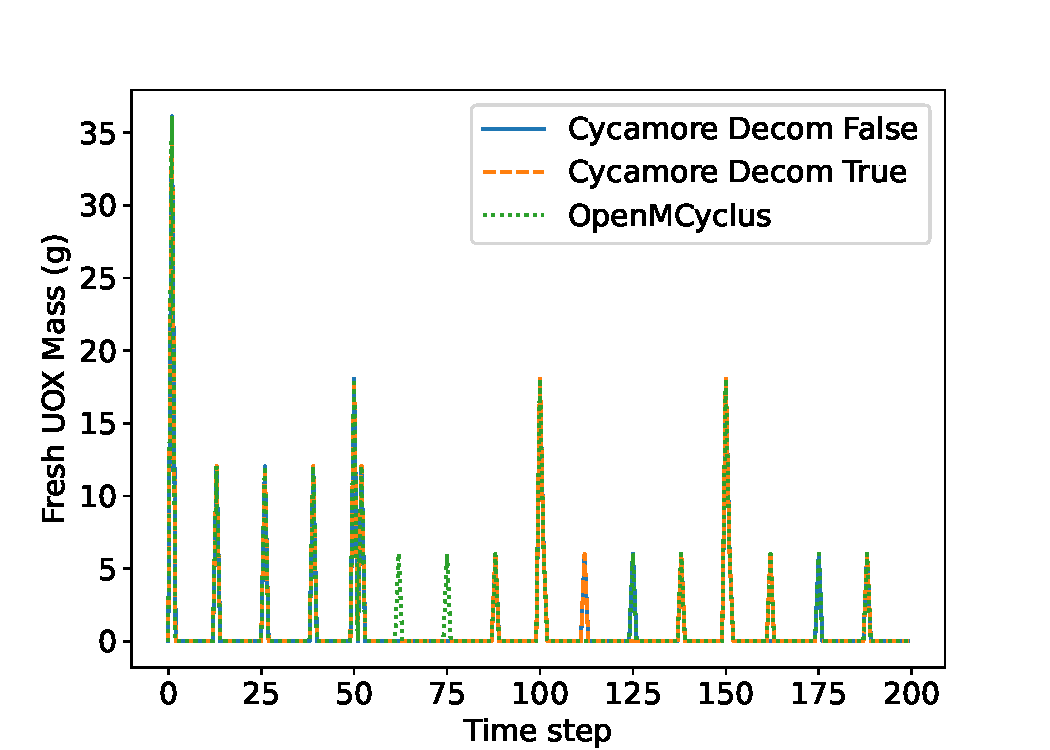
\includegraphics[trim=0 0 30 20,clip,width=\textwidth]{comparison_uox.pdf}
        \caption{Fresh UOX.}
        \label{fig:comparison_uox}
    \end{subfigure}
    \hfill
    \begin{subfigure}[b]{0.48\textwidth}
        \centering
        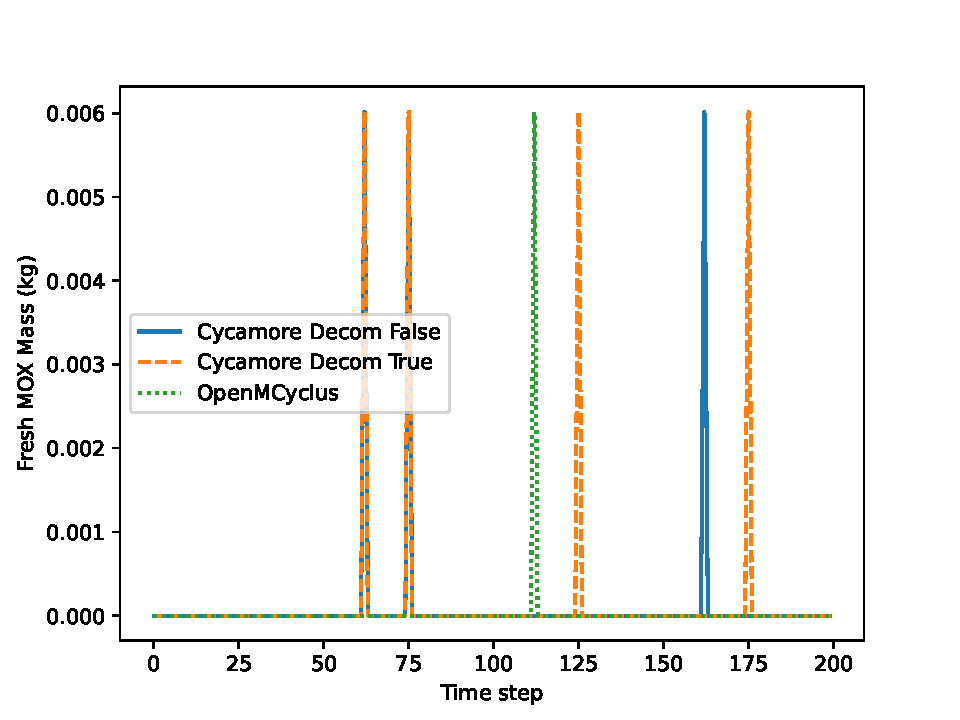
\includegraphics[trim=0 0 30 20,clip,width=\textwidth]{comparison_mox.pdf}
        \caption{Fresh MOX.}
        \label{fig:comparison_mox}
    \end{subfigure}
       \caption{Transactions of the fresh fuel commodities to the 
       reactor facilities when defined with each archetype and 
       setting.}
       \label{fig:comparison_fuel}
\end{figure}

Figure \ref{fig:comparison_spentfuel} shows the transactions of 
spent fuel from the reactors to the separations facility in each 
scenario. There is more variation between the scenarios with the 
\Cycamore \texttt{Reactor} archetype and the scenario with OpenMCyclus. 
The differences in fresh fuel commodities received by the 
reactor facilities propagate to differences in the spent fuel commodity 
discharged by the reactors in each scenario. The timing and quantity of 
fuel traded for non-retirement transactions is consistent between all 
three scenarios, but the commodity type (spent UOX or spent MOX) may 
differ. There are differences in the spent fuel 
transactions that correspond to fuel discharged at the retirement of the 
facilities. The OpenMCyclus archetype discharges all of the assemblies 
in the same time step that the reactor retires. However, the \Cycamore 
\texttt{Reactor} archetype discharges 2/3 of the assemblies in the same 
time step that the facility retires, and the remaining 1/3 of the assemblies 
in the next time step. The behavior of the \Cycamore \texttt{Reactor} 
upon retirement is consistent regardless of the \texttt{decom\_transmute\_all}
setting. This difference in transactions identifies a methodology 
difference between the two archetypes. However, it only affects a 
scenario when a reactor facility is retired, and a one time step difference 
in when the fuel from the core is traded away is not large. Therefore, 
this methodology difference is not expected to lead to large differences 
in the behavior of a scenario. 

\begin{figure}[ht!]
    \centering
    \begin{subfigure}[b]{0.48\textwidth}
        \centering
        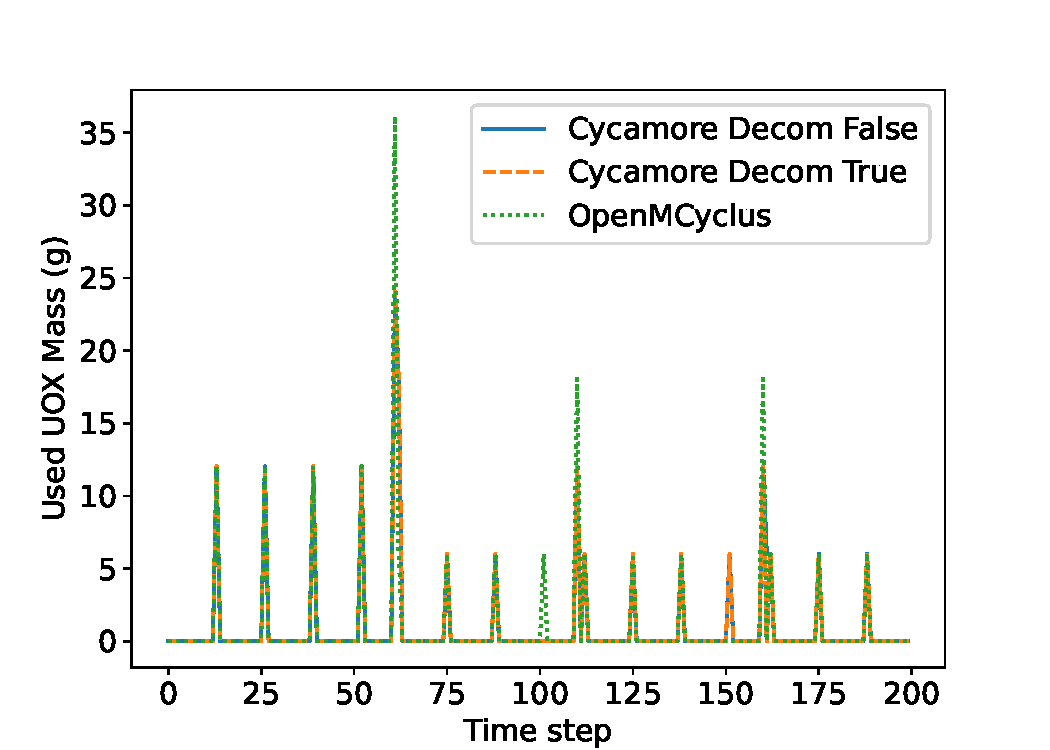
\includegraphics[trim=0 0 30 20,clip,width=\textwidth]{comparison_spentuox.pdf}
        \caption{Spent UOX.}
        \label{fig:comparison_spentuox}
    \end{subfigure}
    \hfill
    \begin{subfigure}[b]{0.48\textwidth}
        \centering
        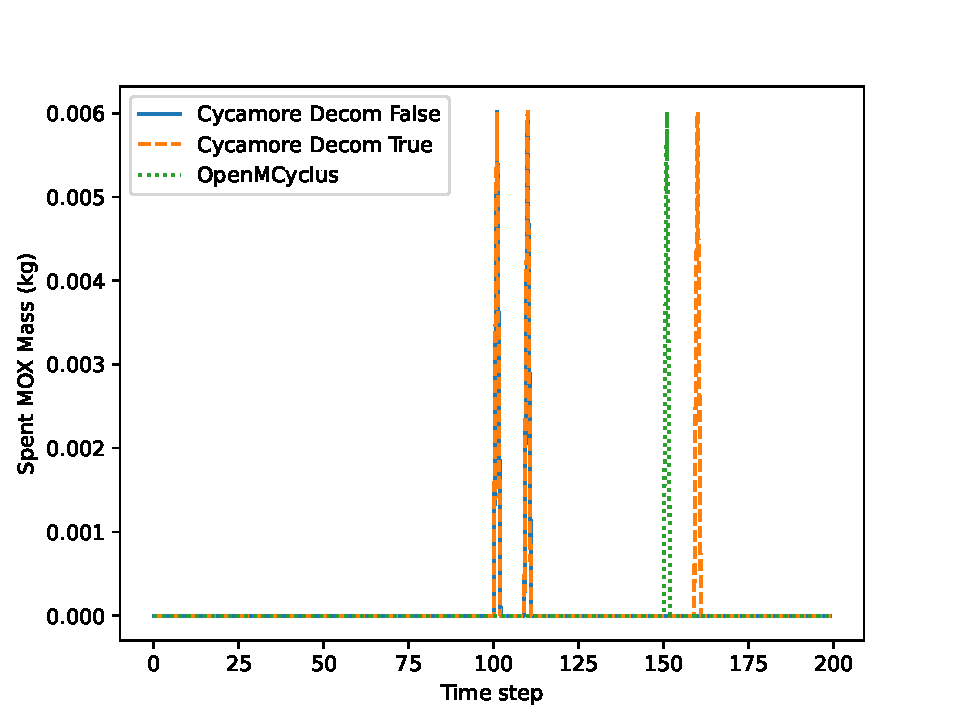
\includegraphics[trim=0 0 30 20,clip,width=\textwidth]{comparison_spentmox.pdf}
        \caption{Spent MOX.}
        \label{fig:comparison_spentmox}
    \end{subfigure}
       \caption{Transactions of the spent fuel commodities from the 
       reactor facilities when defined with each archetype and 
       setting.}
       \label{fig:comparison_spentfuel}
\end{figure}

Finally, Figure \ref{fig:comparison_pu} shows the instantaneous and cumulative 
masses of separated plutonium traded from the separations facility to 
the fuel fabrication facility. Because of the large material capacity of 
the fuel fabrication facility, all of the separated plutonium is traded 
away in the time step after it is separated, so the separations facility does 
not accumulate an inventory of separated plutonium. The three different 
scenarios show consistency
in when the separated plutonium is traded: one time step after a spent
\gls{UOX} assembly is traded to the separations facility. However, the 
amount of plutonium traded varies between the three scenarios. The two 
scenarios that use the \Cycamore \texttt{Reactor} show agreement in the 
traded plutonium mass until time step 61, when the first two reactors are
retired. The disagreement between these two scenarios arises from the 
\texttt{decom\_transmute\_all} setting. When set to \texttt{True}, 
all of the assemblies in the core are transmuted upon retirement, 
while when set to \texttt{False} only half of the assemblies are 
transmuted (in this case two of the three assemblies). Therefore, 
when this setting is \texttt{False}, not all of the 
spent fuel assemblies traded away have the spent fuel composition, and 
there is less plutonium in the defined material compositions 
of the spent fuel assemblies than when all of the assemblies are transmuted. 

\begin{figure}[ht!]
    \centering
    \begin{subfigure}[b]{0.48\textwidth}
        \centering
        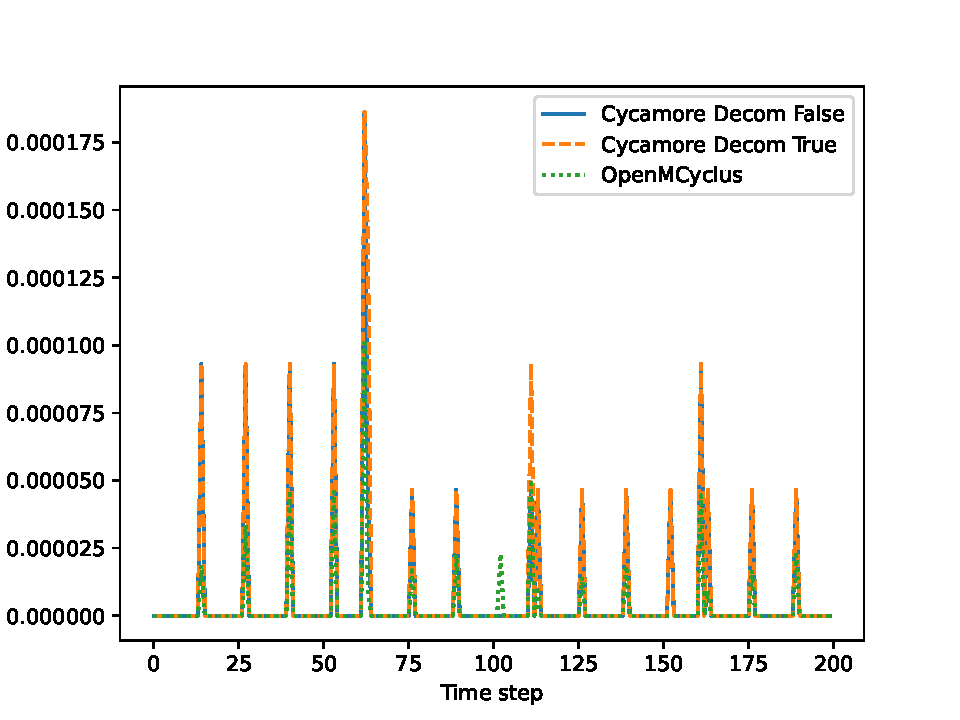
\includegraphics[trim=0 0 30 20,clip,width=\textwidth]{comparison_pu.pdf}
        \caption{Instantaneous plutonium mass}
        \label{fig:comparison_pu_inst}
    \end{subfigure}
    \hfill
    \begin{subfigure}[b]{0.48\textwidth}
        \centering
        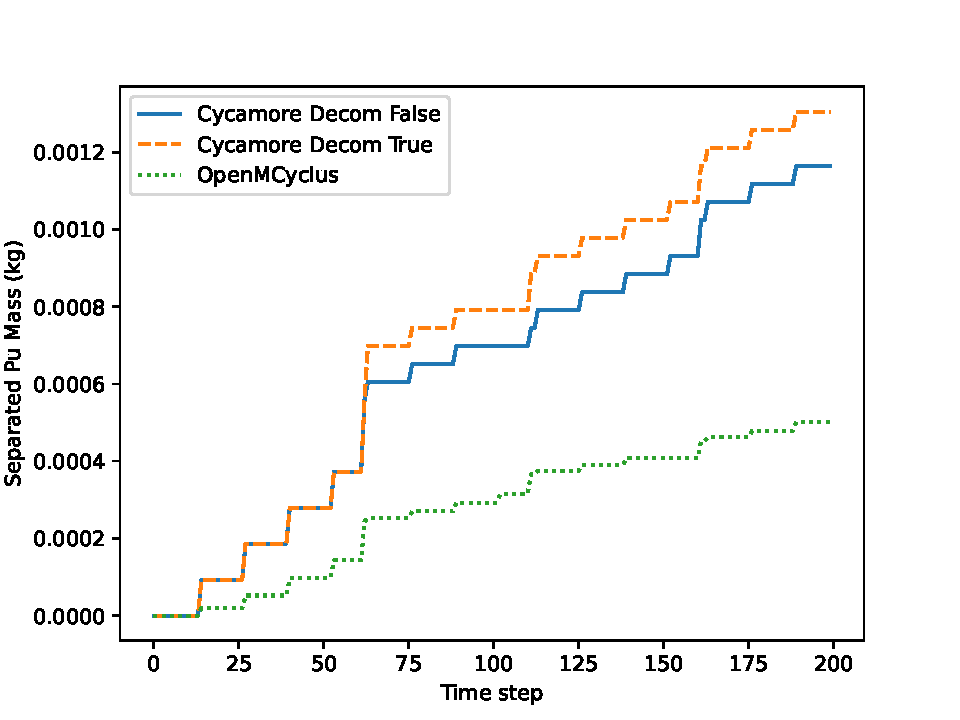
\includegraphics[trim=0 0 30 20,clip,width=\textwidth]{comparison_pu_cumulative.pdf}
        \caption{Cumulative plutonium mass}
        \label{fig:comparison_pu_cumulative}
    \end{subfigure}
       \caption{Transactions of the separated plutonium from the
       separation facility to the fuel fabrication facility, based 
       on the archetype to define the reactor facilities.}
       \label{fig:comparison_pu}
\end{figure}

The differences in traded separated plutonium when using the \Cycamore 
\texttt{Reactor} and OpenMCyclus archetype stems 
primarily from the different methodologies in how the assemblies 
are transmuted. For the spent fuel compositions in the cases with the \Cycamore 
\texttt{Reactor}, we depleted an assembly for an entire residence time 
(36 months continuously). However, in OpenMCyclus the fuel is depleted for 
a single cycle at a time (12 months in this case). Therefore, the 
assemblies discharged at the end of the first two cycles by the 
OpenMCyclus prototypes have not been depleted for the full 36 months 
like they are with the \Cycamore \texttt{Reactor} prototype. To confirm  
that the difference in the time steps of the depletion led to the 
difference in separated plutonium inventory, we temporarily changed
the OpenMCyclus source code to deplete the fuel in a more similar 
manner to that of the \Cycamore \texttt{Reactor}: each assembly was 
depleted for the full 36 month residence time right before being 
discharged. This modification, shown in red in Figure 
\ref{fig:comparison_pu_discharge}, shows that when the assemblies 
are always depleted for the full 36 month duration the 
separated plutonium masses are more consistent with those from 
using the \Cycamore \texttt{Reactor} archetype. The consistency 
between the two archetypes when using the modified OpenMCyclus 
provides confidence in the results of OpenMCyclus when the fuel 
is depleted each cycle instead of upon discharge. 

The transmutation methodologies differences between the archetypes 
led to the differences in the traded plutonium masses, which then 
led to the differences in the type of fresh fuel received by 
the reactors in each scenario. The \Cycamore \texttt{Reactor}
archetype with all of the assemblies transmuted at facility 
decommissioning resulted in this scenario having the most 
fresh \gls{MOX} assemblies sent to the reactors. 

\begin{figure}[ht!]
    \centering
    \begin{subfigure}[b]{0.48\textwidth}
        \centering
        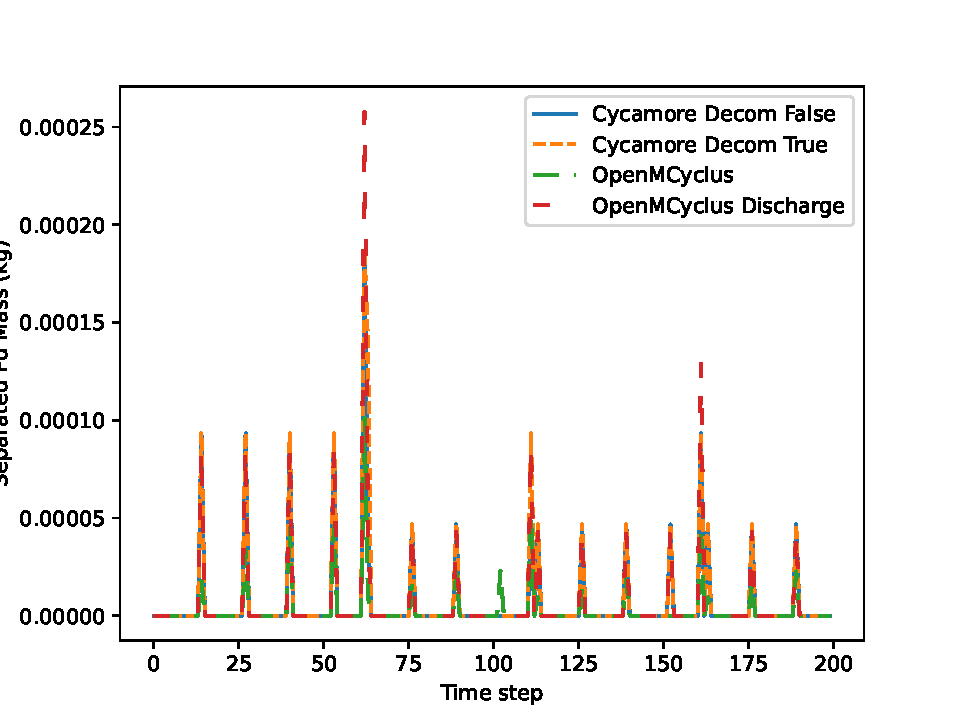
\includegraphics[trim=0 0 30 20,clip,width=\textwidth]{comparison_pu_discharge.pdf}
        \caption{Instantaneous plutonium mass}
        \label{fig:comparison_pu_inst_discharge}
    \end{subfigure}
    \hfill
    \begin{subfigure}[b]{0.48\textwidth}
        \centering
        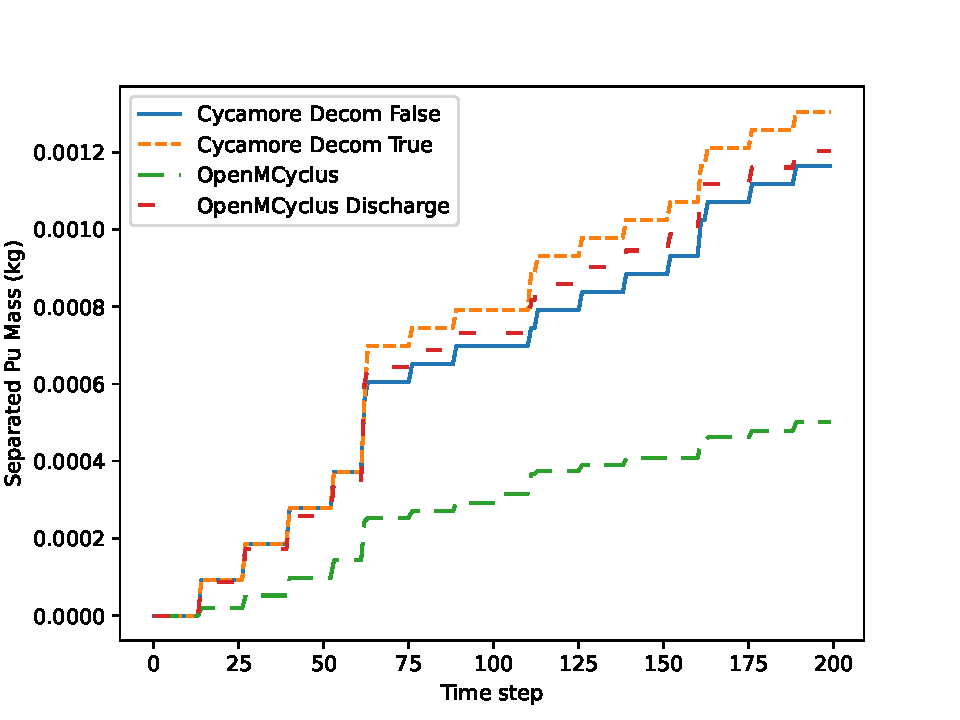
\includegraphics[trim=0 0 30 20,clip,width=\textwidth]{comparison_pu_cumulative_discharge.pdf}
        \caption{Cumulative plutonium mass}
        \label{fig:comparison_pu_cumulative_discharge}
    \end{subfigure}
       \caption{Transactions of the separated plutonium from the
       separation facility to the fuel fabrication facility, based 
       on the archetype to define the reactor facilities.}
       \label{fig:comparison_pu_discharge}
\end{figure}
